\documentclass[twoside]{book}

% Packages required by doxygen
\usepackage{fixltx2e}
\usepackage{calc}
\usepackage{doxygen}
\usepackage[export]{adjustbox} % also loads graphicx
\usepackage{graphicx}
\usepackage[utf8]{inputenc}
\usepackage{makeidx}
\usepackage{multicol}
\usepackage{multirow}
\PassOptionsToPackage{warn}{textcomp}
\usepackage{textcomp}
\usepackage[nointegrals]{wasysym}
\usepackage[table]{xcolor}

% Font selection
\usepackage[T1]{fontenc}
\usepackage[scaled=.90]{helvet}
\usepackage{courier}
\usepackage{amssymb}
\usepackage{sectsty}
\renewcommand{\familydefault}{\sfdefault}
\allsectionsfont{%
  \fontseries{bc}\selectfont%
  \color{darkgray}%
}
\renewcommand{\DoxyLabelFont}{%
  \fontseries{bc}\selectfont%
  \color{darkgray}%
}
\newcommand{\+}{\discretionary{\mbox{\scriptsize$\hookleftarrow$}}{}{}}

% Page & text layout
\usepackage{geometry}
\geometry{%
  a4paper,%
  top=2.5cm,%
  bottom=2.5cm,%
  left=2.5cm,%
  right=2.5cm%
}
\tolerance=750
\hfuzz=15pt
\hbadness=750
\setlength{\emergencystretch}{15pt}
\setlength{\parindent}{0cm}
\setlength{\parskip}{3ex plus 2ex minus 2ex}
\makeatletter
\renewcommand{\paragraph}{%
  \@startsection{paragraph}{4}{0ex}{-1.0ex}{1.0ex}{%
    \normalfont\normalsize\bfseries\SS@parafont%
  }%
}
\renewcommand{\subparagraph}{%
  \@startsection{subparagraph}{5}{0ex}{-1.0ex}{1.0ex}{%
    \normalfont\normalsize\bfseries\SS@subparafont%
  }%
}
\makeatother

% Headers & footers
\usepackage{fancyhdr}
\pagestyle{fancyplain}
\fancyhead[LE]{\fancyplain{}{\bfseries\thepage}}
\fancyhead[CE]{\fancyplain{}{}}
\fancyhead[RE]{\fancyplain{}{\bfseries\leftmark}}
\fancyhead[LO]{\fancyplain{}{\bfseries\rightmark}}
\fancyhead[CO]{\fancyplain{}{}}
\fancyhead[RO]{\fancyplain{}{\bfseries\thepage}}
\fancyfoot[LE]{\fancyplain{}{}}
\fancyfoot[CE]{\fancyplain{}{}}
\fancyfoot[RE]{\fancyplain{}{\bfseries\scriptsize Generated by Doxygen }}
\fancyfoot[LO]{\fancyplain{}{\bfseries\scriptsize Generated by Doxygen }}
\fancyfoot[CO]{\fancyplain{}{}}
\fancyfoot[RO]{\fancyplain{}{}}
\renewcommand{\footrulewidth}{0.4pt}
\renewcommand{\chaptermark}[1]{%
  \markboth{#1}{}%
}
\renewcommand{\sectionmark}[1]{%
  \markright{\thesection\ #1}%
}

% Indices & bibliography
\usepackage{natbib}
\usepackage[titles]{tocloft}
\setcounter{tocdepth}{3}
\setcounter{secnumdepth}{5}
\makeindex

% Hyperlinks (required, but should be loaded last)
\usepackage{ifpdf}
\ifpdf
  \usepackage[pdftex,pagebackref=true]{hyperref}
\else
  \usepackage[ps2pdf,pagebackref=true]{hyperref}
\fi
\hypersetup{%
  colorlinks=true,%
  linkcolor=blue,%
  citecolor=blue,%
  unicode%
}

% Custom commands
\newcommand{\clearemptydoublepage}{%
  \newpage{\pagestyle{empty}\cleardoublepage}%
}

\usepackage{caption}
\captionsetup{labelsep=space,justification=centering,font={bf},singlelinecheck=off,skip=4pt,position=top}

%===== C O N T E N T S =====

\begin{document}

% Titlepage & ToC
\hypersetup{pageanchor=false,
             bookmarksnumbered=true,
             pdfencoding=unicode
            }
\pagenumbering{alph}
\begin{titlepage}
\vspace*{7cm}
\begin{center}%
{\Large Kinect Security System \\[1ex]\large v1.\+1 }\\
\vspace*{1cm}
{\large Generated by Doxygen 1.8.13}\\
\end{center}
\end{titlepage}
\clearemptydoublepage
\pagenumbering{roman}
\tableofcontents
\clearemptydoublepage
\pagenumbering{arabic}
\hypersetup{pageanchor=true}

%--- Begin generated contents ---
\chapter{Continuous\+Gesture\+Basics-\/\+W\+PF}
\label{md__kinect_security_system__r_e_a_d_m_e}
\Hypertarget{md__kinect_security_system__r_e_a_d_m_e}
Demonstrates how to use Continuous Gestures in Kinect for Windows v2 
\chapter{Namespace Index}
\section{Packages}
Here are the packages with brief descriptions (if available)\+:\begin{DoxyCompactList}
\item\contentsline{section}{\hyperlink{namespace_microsoft}{Microsoft} }{\pageref{namespace_microsoft}}{}
\item\contentsline{section}{\hyperlink{namespace_microsoft_1_1_samples}{Microsoft.\+Samples} }{\pageref{namespace_microsoft_1_1_samples}}{}
\item\contentsline{section}{\hyperlink{namespace_microsoft_1_1_samples_1_1_kinect}{Microsoft.\+Samples.\+Kinect} }{\pageref{namespace_microsoft_1_1_samples_1_1_kinect}}{}
\item\contentsline{section}{\hyperlink{namespace_microsoft_1_1_samples_1_1_kinect_1_1_kinect_security_system}{Microsoft.\+Samples.\+Kinect.\+Kinect\+Security\+System} }{\pageref{namespace_microsoft_1_1_samples_1_1_kinect_1_1_kinect_security_system}}{}
\end{DoxyCompactList}

\chapter{Hierarchical Index}
\section{Class Hierarchy}
This inheritance list is sorted roughly, but not completely, alphabetically\+:\begin{DoxyCompactList}
\item Application\begin{DoxyCompactList}
\item \contentsline{section}{Microsoft.\+Samples.\+Kinect.\+Kinect\+Security\+System.\+App}{\pageref{class_microsoft_1_1_samples_1_1_kinect_1_1_kinect_security_system_1_1_app}}{}
\end{DoxyCompactList}
\item Bindable\+Base\begin{DoxyCompactList}
\item \contentsline{section}{Microsoft.\+Samples.\+Kinect.\+Kinect\+Security\+System.\+Gesture\+Result\+View}{\pageref{class_microsoft_1_1_samples_1_1_kinect_1_1_kinect_security_system_1_1_gesture_result_view}}{}
\item \contentsline{section}{Microsoft.\+Samples.\+Kinect.\+Kinect\+Security\+System.\+Robot\+Control}{\pageref{class_microsoft_1_1_samples_1_1_kinect_1_1_kinect_security_system_1_1_robot_control}}{}
\end{DoxyCompactList}
\item I\+Disposable\begin{DoxyCompactList}
\item \contentsline{section}{Microsoft.\+Samples.\+Kinect.\+Kinect\+Security\+System.\+Gesture\+Detector}{\pageref{class_microsoft_1_1_samples_1_1_kinect_1_1_kinect_security_system_1_1_gesture_detector}}{}
\item \contentsline{section}{Microsoft.\+Samples.\+Kinect.\+Kinect\+Security\+System.\+Main\+Window}{\pageref{class_microsoft_1_1_samples_1_1_kinect_1_1_kinect_security_system_1_1_main_window}}{}
\end{DoxyCompactList}
\item I\+Notify\+Property\+Changed\begin{DoxyCompactList}
\item \contentsline{section}{Microsoft.\+Samples.\+Kinect.\+Kinect\+Security\+System.\+Main\+Window}{\pageref{class_microsoft_1_1_samples_1_1_kinect_1_1_kinect_security_system_1_1_main_window}}{}
\end{DoxyCompactList}
\item \contentsline{section}{Microsoft.\+Samples.\+Kinect.\+Kinect\+Security\+System.\+Kinect\+Body\+View}{\pageref{class_microsoft_1_1_samples_1_1_kinect_1_1_kinect_security_system_1_1_kinect_body_view}}{}
\item Window\begin{DoxyCompactList}
\item \contentsline{section}{Microsoft.\+Samples.\+Kinect.\+Kinect\+Security\+System.\+Main\+Window}{\pageref{class_microsoft_1_1_samples_1_1_kinect_1_1_kinect_security_system_1_1_main_window}}{}
\end{DoxyCompactList}
\end{DoxyCompactList}

\chapter{Class Index}
\section{Class List}
Here are the classes, structs, unions and interfaces with brief descriptions\+:\begin{DoxyCompactList}
\item\contentsline{section}{\hyperlink{class_microsoft_1_1_samples_1_1_kinect_1_1_kinect_security_system_1_1_app}{Microsoft.\+Samples.\+Kinect.\+Kinect\+Security\+System.\+App} \\*Interaction logic for \hyperlink{class_microsoft_1_1_samples_1_1_kinect_1_1_kinect_security_system_1_1_app}{App} }{\pageref{class_microsoft_1_1_samples_1_1_kinect_1_1_kinect_security_system_1_1_app}}{}
\item\contentsline{section}{\hyperlink{class_microsoft_1_1_samples_1_1_kinect_1_1_kinect_security_system_1_1_gesture_detector}{Microsoft.\+Samples.\+Kinect.\+Kinect\+Security\+System.\+Gesture\+Detector} \\*Gesture Detector class which polls for Visual\+Gesture\+Builder\+Frames from the \hyperlink{namespace_microsoft_1_1_samples_1_1_kinect}{Kinect} sensor Updates the associated \hyperlink{class_microsoft_1_1_samples_1_1_kinect_1_1_kinect_security_system_1_1_gesture_result_view}{Gesture\+Result\+View} object with the latest gesture results }{\pageref{class_microsoft_1_1_samples_1_1_kinect_1_1_kinect_security_system_1_1_gesture_detector}}{}
\item\contentsline{section}{\hyperlink{class_microsoft_1_1_samples_1_1_kinect_1_1_kinect_security_system_1_1_gesture_result_view}{Microsoft.\+Samples.\+Kinect.\+Kinect\+Security\+System.\+Gesture\+Result\+View} \\*Tracks gesture results coming from the \hyperlink{class_microsoft_1_1_samples_1_1_kinect_1_1_kinect_security_system_1_1_gesture_detector}{Gesture\+Detector} and displays them in the UI }{\pageref{class_microsoft_1_1_samples_1_1_kinect_1_1_kinect_security_system_1_1_gesture_result_view}}{}
\item\contentsline{section}{\hyperlink{class_microsoft_1_1_samples_1_1_kinect_1_1_kinect_security_system_1_1_kinect_body_view}{Microsoft.\+Samples.\+Kinect.\+Kinect\+Security\+System.\+Kinect\+Body\+View} \\*Visualizes the \hyperlink{namespace_microsoft_1_1_samples_1_1_kinect}{Kinect} Body stream for display in the UI }{\pageref{class_microsoft_1_1_samples_1_1_kinect_1_1_kinect_security_system_1_1_kinect_body_view}}{}
\item\contentsline{section}{\hyperlink{class_microsoft_1_1_samples_1_1_kinect_1_1_kinect_security_system_1_1_main_window}{Microsoft.\+Samples.\+Kinect.\+Kinect\+Security\+System.\+Main\+Window} \\*Interaction logic for the \hyperlink{class_microsoft_1_1_samples_1_1_kinect_1_1_kinect_security_system_1_1_main_window}{Main\+Window} }{\pageref{class_microsoft_1_1_samples_1_1_kinect_1_1_kinect_security_system_1_1_main_window}}{}
\item\contentsline{section}{\hyperlink{class_microsoft_1_1_samples_1_1_kinect_1_1_kinect_security_system_1_1_robot_control}{Microsoft.\+Samples.\+Kinect.\+Kinect\+Security\+System.\+Robot\+Control} \\*Holds the logic for controlling the robot arm using skeleton tracking }{\pageref{class_microsoft_1_1_samples_1_1_kinect_1_1_kinect_security_system_1_1_robot_control}}{}
\end{DoxyCompactList}

\chapter{Namespace Documentation}
\hypertarget{namespace_microsoft}{}\section{Microsoft Namespace Reference}
\label{namespace_microsoft}\index{Microsoft@{Microsoft}}
\subsection*{Namespaces}
\begin{DoxyCompactItemize}
\end{DoxyCompactItemize}

\hypertarget{namespace_microsoft_1_1_samples}{}\section{Microsoft.\+Samples Namespace Reference}
\label{namespace_microsoft_1_1_samples}\index{Microsoft.\+Samples@{Microsoft.\+Samples}}
\subsection*{Namespaces}
\begin{DoxyCompactItemize}
\end{DoxyCompactItemize}

\hypertarget{namespace_microsoft_1_1_samples_1_1_kinect}{}\section{Microsoft.\+Samples.\+Kinect Namespace Reference}
\label{namespace_microsoft_1_1_samples_1_1_kinect}\index{Microsoft.\+Samples.\+Kinect@{Microsoft.\+Samples.\+Kinect}}
\subsection*{Namespaces}
\begin{DoxyCompactItemize}
\end{DoxyCompactItemize}

\hypertarget{namespace_microsoft_1_1_samples_1_1_kinect_1_1_kinect_security_system}{}\section{Microsoft.\+Samples.\+Kinect.\+Kinect\+Security\+System Namespace Reference}
\label{namespace_microsoft_1_1_samples_1_1_kinect_1_1_kinect_security_system}\index{Microsoft.\+Samples.\+Kinect.\+Kinect\+Security\+System@{Microsoft.\+Samples.\+Kinect.\+Kinect\+Security\+System}}
\subsection*{Classes}
\begin{DoxyCompactItemize}
\item 
class \hyperlink{class_microsoft_1_1_samples_1_1_kinect_1_1_kinect_security_system_1_1_app}{App}
\begin{DoxyCompactList}\small\item\em Interaction logic for \hyperlink{class_microsoft_1_1_samples_1_1_kinect_1_1_kinect_security_system_1_1_app}{App} \end{DoxyCompactList}\item 
class \hyperlink{class_microsoft_1_1_samples_1_1_kinect_1_1_kinect_security_system_1_1_gesture_detector}{Gesture\+Detector}
\begin{DoxyCompactList}\small\item\em Gesture Detector class which polls for Visual\+Gesture\+Builder\+Frames from the \hyperlink{namespace_microsoft_1_1_samples_1_1_kinect}{Kinect} sensor Updates the associated \hyperlink{class_microsoft_1_1_samples_1_1_kinect_1_1_kinect_security_system_1_1_gesture_result_view}{Gesture\+Result\+View} object with the latest gesture results \end{DoxyCompactList}\item 
class \hyperlink{class_microsoft_1_1_samples_1_1_kinect_1_1_kinect_security_system_1_1_gesture_result_view}{Gesture\+Result\+View}
\begin{DoxyCompactList}\small\item\em Tracks gesture results coming from the \hyperlink{class_microsoft_1_1_samples_1_1_kinect_1_1_kinect_security_system_1_1_gesture_detector}{Gesture\+Detector} and displays them in the UI. \end{DoxyCompactList}\item 
class \hyperlink{class_microsoft_1_1_samples_1_1_kinect_1_1_kinect_security_system_1_1_kinect_body_view}{Kinect\+Body\+View}
\begin{DoxyCompactList}\small\item\em Visualizes the \hyperlink{namespace_microsoft_1_1_samples_1_1_kinect}{Kinect} Body stream for display in the UI \end{DoxyCompactList}\item 
class \hyperlink{class_microsoft_1_1_samples_1_1_kinect_1_1_kinect_security_system_1_1_main_window}{Main\+Window}
\begin{DoxyCompactList}\small\item\em Interaction logic for the \hyperlink{class_microsoft_1_1_samples_1_1_kinect_1_1_kinect_security_system_1_1_main_window}{Main\+Window} \end{DoxyCompactList}\item 
class \hyperlink{class_microsoft_1_1_samples_1_1_kinect_1_1_kinect_security_system_1_1_robot_control}{Robot\+Control}
\begin{DoxyCompactList}\small\item\em Holds the logic for controlling the robot arm using skeleton tracking \end{DoxyCompactList}\end{DoxyCompactItemize}

\chapter{Class Documentation}
\hypertarget{class_microsoft_1_1_samples_1_1_kinect_1_1_kinect_security_system_1_1_app}{}\section{Microsoft.\+Samples.\+Kinect.\+Kinect\+Security\+System.\+App Class Reference}
\label{class_microsoft_1_1_samples_1_1_kinect_1_1_kinect_security_system_1_1_app}\index{Microsoft.\+Samples.\+Kinect.\+Kinect\+Security\+System.\+App@{Microsoft.\+Samples.\+Kinect.\+Kinect\+Security\+System.\+App}}


Interaction logic for \hyperlink{class_microsoft_1_1_samples_1_1_kinect_1_1_kinect_security_system_1_1_app}{App}  


Inheritance diagram for Microsoft.\+Samples.\+Kinect.\+Kinect\+Security\+System.\+App\+:\begin{figure}[H]
\begin{center}
\leavevmode
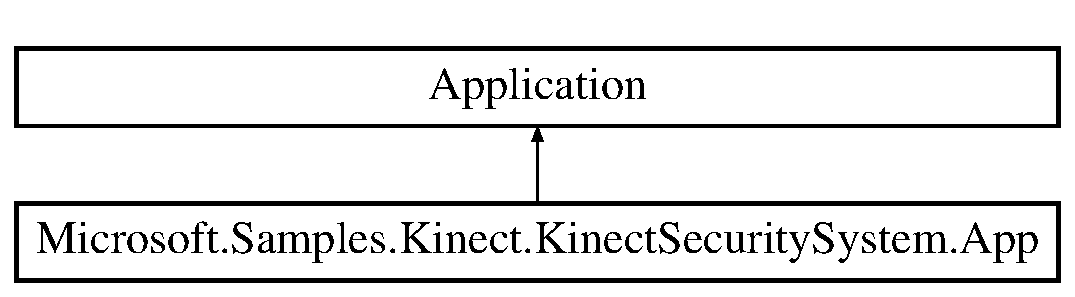
\includegraphics[height=2.000000cm]{class_microsoft_1_1_samples_1_1_kinect_1_1_kinect_security_system_1_1_app}
\end{center}
\end{figure}


\subsection{Detailed Description}
Interaction logic for \hyperlink{class_microsoft_1_1_samples_1_1_kinect_1_1_kinect_security_system_1_1_app}{App} 



The documentation for this class was generated from the following file\+:\begin{DoxyCompactItemize}
\item 
Kinect\+Security\+System/App.\+xaml.\+cs\end{DoxyCompactItemize}

\hypertarget{class_microsoft_1_1_samples_1_1_kinect_1_1_kinect_security_system_1_1_gesture_detector}{}\section{Microsoft.\+Samples.\+Kinect.\+Kinect\+Security\+System.\+Gesture\+Detector Class Reference}
\label{class_microsoft_1_1_samples_1_1_kinect_1_1_kinect_security_system_1_1_gesture_detector}\index{Microsoft.\+Samples.\+Kinect.\+Kinect\+Security\+System.\+Gesture\+Detector@{Microsoft.\+Samples.\+Kinect.\+Kinect\+Security\+System.\+Gesture\+Detector}}


Gesture Detector class which polls for Visual\+Gesture\+Builder\+Frames from the \hyperlink{namespace_microsoft_1_1_samples_1_1_kinect}{Kinect} sensor Updates the associated \hyperlink{class_microsoft_1_1_samples_1_1_kinect_1_1_kinect_security_system_1_1_gesture_result_view}{Gesture\+Result\+View} object with the latest gesture results  


Inheritance diagram for Microsoft.\+Samples.\+Kinect.\+Kinect\+Security\+System.\+Gesture\+Detector\+:\begin{figure}[H]
\begin{center}
\leavevmode
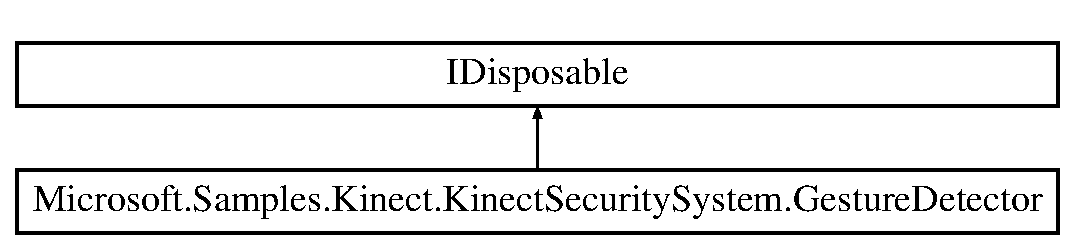
\includegraphics[height=2.000000cm]{class_microsoft_1_1_samples_1_1_kinect_1_1_kinect_security_system_1_1_gesture_detector}
\end{center}
\end{figure}
\subsection*{Public Member Functions}
\begin{DoxyCompactItemize}
\item 
void \hyperlink{class_microsoft_1_1_samples_1_1_kinect_1_1_kinect_security_system_1_1_gesture_detector_a605c6a5ff0f3857d5af4d0548d0a8d50}{set\+Gestures} (string gesture1, string gesture2, string gesture3)
\begin{DoxyCompactList}\small\item\em Sets the three gestures used to lock/unlock the system to the parameters \end{DoxyCompactList}\item 
\hyperlink{class_microsoft_1_1_samples_1_1_kinect_1_1_kinect_security_system_1_1_gesture_detector_ac072ff2ebd85a754b9b1b4e925757d8a}{Gesture\+Detector} (Kinect\+Sensor kinect\+Sensor, \hyperlink{class_microsoft_1_1_samples_1_1_kinect_1_1_kinect_security_system_1_1_gesture_result_view}{Gesture\+Result\+View} gesture\+Result\+View)
\begin{DoxyCompactList}\small\item\em Initializes a new instance of the \hyperlink{class_microsoft_1_1_samples_1_1_kinect_1_1_kinect_security_system_1_1_gesture_detector}{Gesture\+Detector} class along with the gesture frame source and reader \end{DoxyCompactList}\item 
void \hyperlink{class_microsoft_1_1_samples_1_1_kinect_1_1_kinect_security_system_1_1_gesture_detector_a37bfd6d98a0d7ef40a4080115cde2946}{force\+U\+I\+U\+Pdate} ()
\begin{DoxyCompactList}\small\item\em Forces the UI to update it\textquotesingle{}s required parameters \end{DoxyCompactList}\item 
void \hyperlink{class_microsoft_1_1_samples_1_1_kinect_1_1_kinect_security_system_1_1_gesture_detector_aa135be3ffe1a256ce8c19eaff88ef37c}{Update\+Gesture\+Data} ()
\begin{DoxyCompactList}\small\item\em Retrieves the latest gesture detection results from the sensor \end{DoxyCompactList}\item 
void \hyperlink{class_microsoft_1_1_samples_1_1_kinect_1_1_kinect_security_system_1_1_gesture_detector_adc6439369c674bc1a9916f851ca15958}{reset\+Sequence} ()
\begin{DoxyCompactList}\small\item\em Resets the current sequence of gestures after a failed attempt, or when changing the unlock sequence \end{DoxyCompactList}\item 
void \hyperlink{class_microsoft_1_1_samples_1_1_kinect_1_1_kinect_security_system_1_1_gesture_detector_aec416d9411b2760f932af8135274c4d8}{Dispose} ()
\begin{DoxyCompactList}\small\item\em Disposes the Visual\+Gesture\+Builder\+Frame\+Source and Visual\+Gesture\+Builder\+Frame\+Reader objects \end{DoxyCompactList}\end{DoxyCompactItemize}
\subsection*{Public Attributes}
\begin{DoxyCompactItemize}
\item 
bool \hyperlink{class_microsoft_1_1_samples_1_1_kinect_1_1_kinect_security_system_1_1_gesture_detector_ae7a78de4832f284933db25aaaad77ce4}{is\+Taking\+Screenshot} = false
\begin{DoxyCompactList}\small\item\em Boolean for checking whether a screenshot needs to be taken for the security alert \end{DoxyCompactList}\end{DoxyCompactItemize}
\subsection*{Properties}
\begin{DoxyCompactItemize}
\item 
\hyperlink{class_microsoft_1_1_samples_1_1_kinect_1_1_kinect_security_system_1_1_gesture_result_view}{Gesture\+Result\+View} \hyperlink{class_microsoft_1_1_samples_1_1_kinect_1_1_kinect_security_system_1_1_gesture_detector_a40558db94165f47ad3526f24d2f52f6c}{Gesture\+Result\+View}\hspace{0.3cm}{\ttfamily  \mbox{[}get\mbox{]}}
\begin{DoxyCompactList}\small\item\em Gets the \hyperlink{class_microsoft_1_1_samples_1_1_kinect_1_1_kinect_security_system_1_1_gesture_result_view}{Gesture\+Result\+View} object which stores the detector results for display in the UI \end{DoxyCompactList}\item 
bool \hyperlink{class_microsoft_1_1_samples_1_1_kinect_1_1_kinect_security_system_1_1_gesture_detector_a4a4d7870b3fe47c605bb336ce8b08e6b}{Closed\+Hand\+State}\hspace{0.3cm}{\ttfamily  \mbox{[}get, set\mbox{]}}
\begin{DoxyCompactList}\small\item\em Gets or sets a value indicating whether the body associated with the detector has at least one hand closed \end{DoxyCompactList}\item 
ulong \hyperlink{class_microsoft_1_1_samples_1_1_kinect_1_1_kinect_security_system_1_1_gesture_detector_a4ea0f9304d3588e60a6d0e8a2832cb9c}{Tracking\+Id}\hspace{0.3cm}{\ttfamily  \mbox{[}get, set\mbox{]}}
\begin{DoxyCompactList}\small\item\em Gets or sets the body tracking ID associated with the current detector The tracking ID can change whenever a body comes in/out of scope \end{DoxyCompactList}\item 
bool \hyperlink{class_microsoft_1_1_samples_1_1_kinect_1_1_kinect_security_system_1_1_gesture_detector_a3cfd7fc3420ca6e027e150b9bc66cd53}{Is\+Paused}\hspace{0.3cm}{\ttfamily  \mbox{[}get, set\mbox{]}}
\begin{DoxyCompactList}\small\item\em Gets or sets a value indicating whether or not the detector is currently paused If the body tracking ID associated with the detector is not valid, then the detector should be paused \end{DoxyCompactList}\end{DoxyCompactItemize}


\subsection{Detailed Description}
Gesture Detector class which polls for Visual\+Gesture\+Builder\+Frames from the \hyperlink{namespace_microsoft_1_1_samples_1_1_kinect}{Kinect} sensor Updates the associated \hyperlink{class_microsoft_1_1_samples_1_1_kinect_1_1_kinect_security_system_1_1_gesture_result_view}{Gesture\+Result\+View} object with the latest gesture results 



\subsection{Constructor \& Destructor Documentation}
\mbox{\Hypertarget{class_microsoft_1_1_samples_1_1_kinect_1_1_kinect_security_system_1_1_gesture_detector_ac072ff2ebd85a754b9b1b4e925757d8a}\label{class_microsoft_1_1_samples_1_1_kinect_1_1_kinect_security_system_1_1_gesture_detector_ac072ff2ebd85a754b9b1b4e925757d8a}} 
\index{Microsoft\+::\+Samples\+::\+Kinect\+::\+Kinect\+Security\+System\+::\+Gesture\+Detector@{Microsoft\+::\+Samples\+::\+Kinect\+::\+Kinect\+Security\+System\+::\+Gesture\+Detector}!Gesture\+Detector@{Gesture\+Detector}}
\index{Gesture\+Detector@{Gesture\+Detector}!Microsoft\+::\+Samples\+::\+Kinect\+::\+Kinect\+Security\+System\+::\+Gesture\+Detector@{Microsoft\+::\+Samples\+::\+Kinect\+::\+Kinect\+Security\+System\+::\+Gesture\+Detector}}
\subsubsection{\texorpdfstring{Gesture\+Detector()}{GestureDetector()}}
{\footnotesize\ttfamily Microsoft.\+Samples.\+Kinect.\+Kinect\+Security\+System.\+Gesture\+Detector.\+Gesture\+Detector (\begin{DoxyParamCaption}\item[{Kinect\+Sensor}]{kinect\+Sensor,  }\item[{\hyperlink{class_microsoft_1_1_samples_1_1_kinect_1_1_kinect_security_system_1_1_gesture_result_view}{Gesture\+Result\+View}}]{gesture\+Result\+View }\end{DoxyParamCaption})}



Initializes a new instance of the \hyperlink{class_microsoft_1_1_samples_1_1_kinect_1_1_kinect_security_system_1_1_gesture_detector}{Gesture\+Detector} class along with the gesture frame source and reader 


\begin{DoxyParams}{Parameters}
{\em kinect\+Sensor} & Active sensor to initialize the Visual\+Gesture\+Builder\+Frame\+Source object with\\
\hline
{\em gesture\+Result\+View} & \hyperlink{class_microsoft_1_1_samples_1_1_kinect_1_1_kinect_security_system_1_1_gesture_result_view}{Gesture\+Result\+View} object to store gesture results of a single body to\\
\hline
\end{DoxyParams}


\subsection{Member Function Documentation}
\mbox{\Hypertarget{class_microsoft_1_1_samples_1_1_kinect_1_1_kinect_security_system_1_1_gesture_detector_aec416d9411b2760f932af8135274c4d8}\label{class_microsoft_1_1_samples_1_1_kinect_1_1_kinect_security_system_1_1_gesture_detector_aec416d9411b2760f932af8135274c4d8}} 
\index{Microsoft\+::\+Samples\+::\+Kinect\+::\+Kinect\+Security\+System\+::\+Gesture\+Detector@{Microsoft\+::\+Samples\+::\+Kinect\+::\+Kinect\+Security\+System\+::\+Gesture\+Detector}!Dispose@{Dispose}}
\index{Dispose@{Dispose}!Microsoft\+::\+Samples\+::\+Kinect\+::\+Kinect\+Security\+System\+::\+Gesture\+Detector@{Microsoft\+::\+Samples\+::\+Kinect\+::\+Kinect\+Security\+System\+::\+Gesture\+Detector}}
\subsubsection{\texorpdfstring{Dispose()}{Dispose()}}
{\footnotesize\ttfamily void Microsoft.\+Samples.\+Kinect.\+Kinect\+Security\+System.\+Gesture\+Detector.\+Dispose (\begin{DoxyParamCaption}{ }\end{DoxyParamCaption})}



Disposes the Visual\+Gesture\+Builder\+Frame\+Source and Visual\+Gesture\+Builder\+Frame\+Reader objects 

\mbox{\Hypertarget{class_microsoft_1_1_samples_1_1_kinect_1_1_kinect_security_system_1_1_gesture_detector_a37bfd6d98a0d7ef40a4080115cde2946}\label{class_microsoft_1_1_samples_1_1_kinect_1_1_kinect_security_system_1_1_gesture_detector_a37bfd6d98a0d7ef40a4080115cde2946}} 
\index{Microsoft\+::\+Samples\+::\+Kinect\+::\+Kinect\+Security\+System\+::\+Gesture\+Detector@{Microsoft\+::\+Samples\+::\+Kinect\+::\+Kinect\+Security\+System\+::\+Gesture\+Detector}!force\+U\+I\+U\+Pdate@{force\+U\+I\+U\+Pdate}}
\index{force\+U\+I\+U\+Pdate@{force\+U\+I\+U\+Pdate}!Microsoft\+::\+Samples\+::\+Kinect\+::\+Kinect\+Security\+System\+::\+Gesture\+Detector@{Microsoft\+::\+Samples\+::\+Kinect\+::\+Kinect\+Security\+System\+::\+Gesture\+Detector}}
\subsubsection{\texorpdfstring{force\+U\+I\+U\+Pdate()}{forceUIUPdate()}}
{\footnotesize\ttfamily void Microsoft.\+Samples.\+Kinect.\+Kinect\+Security\+System.\+Gesture\+Detector.\+force\+U\+I\+U\+Pdate (\begin{DoxyParamCaption}{ }\end{DoxyParamCaption})}



Forces the UI to update it\textquotesingle{}s required parameters 

\mbox{\Hypertarget{class_microsoft_1_1_samples_1_1_kinect_1_1_kinect_security_system_1_1_gesture_detector_adc6439369c674bc1a9916f851ca15958}\label{class_microsoft_1_1_samples_1_1_kinect_1_1_kinect_security_system_1_1_gesture_detector_adc6439369c674bc1a9916f851ca15958}} 
\index{Microsoft\+::\+Samples\+::\+Kinect\+::\+Kinect\+Security\+System\+::\+Gesture\+Detector@{Microsoft\+::\+Samples\+::\+Kinect\+::\+Kinect\+Security\+System\+::\+Gesture\+Detector}!reset\+Sequence@{reset\+Sequence}}
\index{reset\+Sequence@{reset\+Sequence}!Microsoft\+::\+Samples\+::\+Kinect\+::\+Kinect\+Security\+System\+::\+Gesture\+Detector@{Microsoft\+::\+Samples\+::\+Kinect\+::\+Kinect\+Security\+System\+::\+Gesture\+Detector}}
\subsubsection{\texorpdfstring{reset\+Sequence()}{resetSequence()}}
{\footnotesize\ttfamily void Microsoft.\+Samples.\+Kinect.\+Kinect\+Security\+System.\+Gesture\+Detector.\+reset\+Sequence (\begin{DoxyParamCaption}{ }\end{DoxyParamCaption})}



Resets the current sequence of gestures after a failed attempt, or when changing the unlock sequence 

\mbox{\Hypertarget{class_microsoft_1_1_samples_1_1_kinect_1_1_kinect_security_system_1_1_gesture_detector_a605c6a5ff0f3857d5af4d0548d0a8d50}\label{class_microsoft_1_1_samples_1_1_kinect_1_1_kinect_security_system_1_1_gesture_detector_a605c6a5ff0f3857d5af4d0548d0a8d50}} 
\index{Microsoft\+::\+Samples\+::\+Kinect\+::\+Kinect\+Security\+System\+::\+Gesture\+Detector@{Microsoft\+::\+Samples\+::\+Kinect\+::\+Kinect\+Security\+System\+::\+Gesture\+Detector}!set\+Gestures@{set\+Gestures}}
\index{set\+Gestures@{set\+Gestures}!Microsoft\+::\+Samples\+::\+Kinect\+::\+Kinect\+Security\+System\+::\+Gesture\+Detector@{Microsoft\+::\+Samples\+::\+Kinect\+::\+Kinect\+Security\+System\+::\+Gesture\+Detector}}
\subsubsection{\texorpdfstring{set\+Gestures()}{setGestures()}}
{\footnotesize\ttfamily void Microsoft.\+Samples.\+Kinect.\+Kinect\+Security\+System.\+Gesture\+Detector.\+set\+Gestures (\begin{DoxyParamCaption}\item[{string}]{gesture1,  }\item[{string}]{gesture2,  }\item[{string}]{gesture3 }\end{DoxyParamCaption})}



Sets the three gestures used to lock/unlock the system to the parameters 


\begin{DoxyParams}{Parameters}
{\em gesture1} & \\
\hline
{\em gesture2} & \\
\hline
{\em gesture3} & \\
\hline
\end{DoxyParams}
\mbox{\Hypertarget{class_microsoft_1_1_samples_1_1_kinect_1_1_kinect_security_system_1_1_gesture_detector_aa135be3ffe1a256ce8c19eaff88ef37c}\label{class_microsoft_1_1_samples_1_1_kinect_1_1_kinect_security_system_1_1_gesture_detector_aa135be3ffe1a256ce8c19eaff88ef37c}} 
\index{Microsoft\+::\+Samples\+::\+Kinect\+::\+Kinect\+Security\+System\+::\+Gesture\+Detector@{Microsoft\+::\+Samples\+::\+Kinect\+::\+Kinect\+Security\+System\+::\+Gesture\+Detector}!Update\+Gesture\+Data@{Update\+Gesture\+Data}}
\index{Update\+Gesture\+Data@{Update\+Gesture\+Data}!Microsoft\+::\+Samples\+::\+Kinect\+::\+Kinect\+Security\+System\+::\+Gesture\+Detector@{Microsoft\+::\+Samples\+::\+Kinect\+::\+Kinect\+Security\+System\+::\+Gesture\+Detector}}
\subsubsection{\texorpdfstring{Update\+Gesture\+Data()}{UpdateGestureData()}}
{\footnotesize\ttfamily void Microsoft.\+Samples.\+Kinect.\+Kinect\+Security\+System.\+Gesture\+Detector.\+Update\+Gesture\+Data (\begin{DoxyParamCaption}{ }\end{DoxyParamCaption})}



Retrieves the latest gesture detection results from the sensor 



\subsection{Member Data Documentation}
\mbox{\Hypertarget{class_microsoft_1_1_samples_1_1_kinect_1_1_kinect_security_system_1_1_gesture_detector_ae7a78de4832f284933db25aaaad77ce4}\label{class_microsoft_1_1_samples_1_1_kinect_1_1_kinect_security_system_1_1_gesture_detector_ae7a78de4832f284933db25aaaad77ce4}} 
\index{Microsoft\+::\+Samples\+::\+Kinect\+::\+Kinect\+Security\+System\+::\+Gesture\+Detector@{Microsoft\+::\+Samples\+::\+Kinect\+::\+Kinect\+Security\+System\+::\+Gesture\+Detector}!is\+Taking\+Screenshot@{is\+Taking\+Screenshot}}
\index{is\+Taking\+Screenshot@{is\+Taking\+Screenshot}!Microsoft\+::\+Samples\+::\+Kinect\+::\+Kinect\+Security\+System\+::\+Gesture\+Detector@{Microsoft\+::\+Samples\+::\+Kinect\+::\+Kinect\+Security\+System\+::\+Gesture\+Detector}}
\subsubsection{\texorpdfstring{is\+Taking\+Screenshot}{isTakingScreenshot}}
{\footnotesize\ttfamily bool Microsoft.\+Samples.\+Kinect.\+Kinect\+Security\+System.\+Gesture\+Detector.\+is\+Taking\+Screenshot = false}



Boolean for checking whether a screenshot needs to be taken for the security alert 



\subsection{Property Documentation}
\mbox{\Hypertarget{class_microsoft_1_1_samples_1_1_kinect_1_1_kinect_security_system_1_1_gesture_detector_a4a4d7870b3fe47c605bb336ce8b08e6b}\label{class_microsoft_1_1_samples_1_1_kinect_1_1_kinect_security_system_1_1_gesture_detector_a4a4d7870b3fe47c605bb336ce8b08e6b}} 
\index{Microsoft\+::\+Samples\+::\+Kinect\+::\+Kinect\+Security\+System\+::\+Gesture\+Detector@{Microsoft\+::\+Samples\+::\+Kinect\+::\+Kinect\+Security\+System\+::\+Gesture\+Detector}!Closed\+Hand\+State@{Closed\+Hand\+State}}
\index{Closed\+Hand\+State@{Closed\+Hand\+State}!Microsoft\+::\+Samples\+::\+Kinect\+::\+Kinect\+Security\+System\+::\+Gesture\+Detector@{Microsoft\+::\+Samples\+::\+Kinect\+::\+Kinect\+Security\+System\+::\+Gesture\+Detector}}
\subsubsection{\texorpdfstring{Closed\+Hand\+State}{ClosedHandState}}
{\footnotesize\ttfamily bool Microsoft.\+Samples.\+Kinect.\+Kinect\+Security\+System.\+Gesture\+Detector.\+Closed\+Hand\+State\hspace{0.3cm}{\ttfamily [get]}, {\ttfamily [set]}}



Gets or sets a value indicating whether the body associated with the detector has at least one hand closed 

\mbox{\Hypertarget{class_microsoft_1_1_samples_1_1_kinect_1_1_kinect_security_system_1_1_gesture_detector_a40558db94165f47ad3526f24d2f52f6c}\label{class_microsoft_1_1_samples_1_1_kinect_1_1_kinect_security_system_1_1_gesture_detector_a40558db94165f47ad3526f24d2f52f6c}} 
\index{Microsoft\+::\+Samples\+::\+Kinect\+::\+Kinect\+Security\+System\+::\+Gesture\+Detector@{Microsoft\+::\+Samples\+::\+Kinect\+::\+Kinect\+Security\+System\+::\+Gesture\+Detector}!Gesture\+Result\+View@{Gesture\+Result\+View}}
\index{Gesture\+Result\+View@{Gesture\+Result\+View}!Microsoft\+::\+Samples\+::\+Kinect\+::\+Kinect\+Security\+System\+::\+Gesture\+Detector@{Microsoft\+::\+Samples\+::\+Kinect\+::\+Kinect\+Security\+System\+::\+Gesture\+Detector}}
\subsubsection{\texorpdfstring{Gesture\+Result\+View}{GestureResultView}}
{\footnotesize\ttfamily \hyperlink{class_microsoft_1_1_samples_1_1_kinect_1_1_kinect_security_system_1_1_gesture_result_view}{Gesture\+Result\+View} Microsoft.\+Samples.\+Kinect.\+Kinect\+Security\+System.\+Gesture\+Detector.\+Gesture\+Result\+View\hspace{0.3cm}{\ttfamily [get]}}



Gets the \hyperlink{class_microsoft_1_1_samples_1_1_kinect_1_1_kinect_security_system_1_1_gesture_result_view}{Gesture\+Result\+View} object which stores the detector results for display in the UI 

\mbox{\Hypertarget{class_microsoft_1_1_samples_1_1_kinect_1_1_kinect_security_system_1_1_gesture_detector_a3cfd7fc3420ca6e027e150b9bc66cd53}\label{class_microsoft_1_1_samples_1_1_kinect_1_1_kinect_security_system_1_1_gesture_detector_a3cfd7fc3420ca6e027e150b9bc66cd53}} 
\index{Microsoft\+::\+Samples\+::\+Kinect\+::\+Kinect\+Security\+System\+::\+Gesture\+Detector@{Microsoft\+::\+Samples\+::\+Kinect\+::\+Kinect\+Security\+System\+::\+Gesture\+Detector}!Is\+Paused@{Is\+Paused}}
\index{Is\+Paused@{Is\+Paused}!Microsoft\+::\+Samples\+::\+Kinect\+::\+Kinect\+Security\+System\+::\+Gesture\+Detector@{Microsoft\+::\+Samples\+::\+Kinect\+::\+Kinect\+Security\+System\+::\+Gesture\+Detector}}
\subsubsection{\texorpdfstring{Is\+Paused}{IsPaused}}
{\footnotesize\ttfamily bool Microsoft.\+Samples.\+Kinect.\+Kinect\+Security\+System.\+Gesture\+Detector.\+Is\+Paused\hspace{0.3cm}{\ttfamily [get]}, {\ttfamily [set]}}



Gets or sets a value indicating whether or not the detector is currently paused If the body tracking ID associated with the detector is not valid, then the detector should be paused 

\mbox{\Hypertarget{class_microsoft_1_1_samples_1_1_kinect_1_1_kinect_security_system_1_1_gesture_detector_a4ea0f9304d3588e60a6d0e8a2832cb9c}\label{class_microsoft_1_1_samples_1_1_kinect_1_1_kinect_security_system_1_1_gesture_detector_a4ea0f9304d3588e60a6d0e8a2832cb9c}} 
\index{Microsoft\+::\+Samples\+::\+Kinect\+::\+Kinect\+Security\+System\+::\+Gesture\+Detector@{Microsoft\+::\+Samples\+::\+Kinect\+::\+Kinect\+Security\+System\+::\+Gesture\+Detector}!Tracking\+Id@{Tracking\+Id}}
\index{Tracking\+Id@{Tracking\+Id}!Microsoft\+::\+Samples\+::\+Kinect\+::\+Kinect\+Security\+System\+::\+Gesture\+Detector@{Microsoft\+::\+Samples\+::\+Kinect\+::\+Kinect\+Security\+System\+::\+Gesture\+Detector}}
\subsubsection{\texorpdfstring{Tracking\+Id}{TrackingId}}
{\footnotesize\ttfamily ulong Microsoft.\+Samples.\+Kinect.\+Kinect\+Security\+System.\+Gesture\+Detector.\+Tracking\+Id\hspace{0.3cm}{\ttfamily [get]}, {\ttfamily [set]}}



Gets or sets the body tracking ID associated with the current detector The tracking ID can change whenever a body comes in/out of scope 



The documentation for this class was generated from the following file\+:\begin{DoxyCompactItemize}
\item 
Kinect\+Security\+System/Gesture\+Detector.\+cs\end{DoxyCompactItemize}

\hypertarget{class_microsoft_1_1_samples_1_1_kinect_1_1_kinect_security_system_1_1_gesture_result_view}{}\section{Microsoft.\+Samples.\+Kinect.\+Kinect\+Security\+System.\+Gesture\+Result\+View Class Reference}
\label{class_microsoft_1_1_samples_1_1_kinect_1_1_kinect_security_system_1_1_gesture_result_view}\index{Microsoft.\+Samples.\+Kinect.\+Kinect\+Security\+System.\+Gesture\+Result\+View@{Microsoft.\+Samples.\+Kinect.\+Kinect\+Security\+System.\+Gesture\+Result\+View}}


Tracks gesture results coming from the \hyperlink{class_microsoft_1_1_samples_1_1_kinect_1_1_kinect_security_system_1_1_gesture_detector}{Gesture\+Detector} and displays them in the UI.  


Inheritance diagram for Microsoft.\+Samples.\+Kinect.\+Kinect\+Security\+System.\+Gesture\+Result\+View\+:\begin{figure}[H]
\begin{center}
\leavevmode
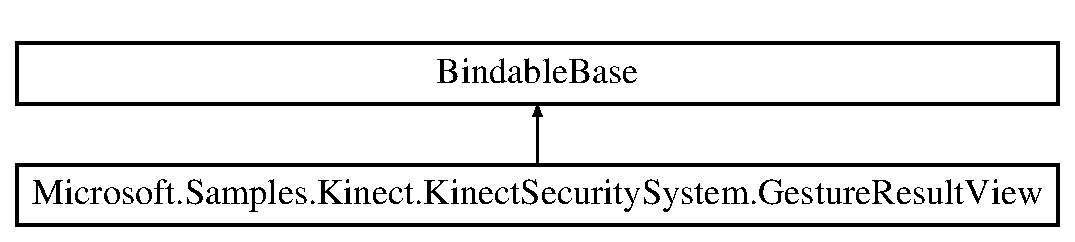
\includegraphics[height=2.000000cm]{class_microsoft_1_1_samples_1_1_kinect_1_1_kinect_security_system_1_1_gesture_result_view}
\end{center}
\end{figure}
\subsection*{Public Member Functions}
\begin{DoxyCompactItemize}
\item 
\hyperlink{class_microsoft_1_1_samples_1_1_kinect_1_1_kinect_security_system_1_1_gesture_result_view_a577bb3cc591276f7128384ca55746126}{Gesture\+Result\+View} (bool is\+Tracked, bool first\+Gesture, bool second\+Gesture, bool third\+Gesture, float progress, bool door\+Unlock\+State, int number\+Of\+Tries, int number\+Of\+Tries\+Left, bool is\+Taking\+Screenshot, bool movement\+Up, bool movement\+Down, bool movement\+Right, bool movement\+Left)
\begin{DoxyCompactList}\small\item\em Initializes a new instance of the \hyperlink{class_microsoft_1_1_samples_1_1_kinect_1_1_kinect_security_system_1_1_gesture_result_view}{Gesture\+Result\+View} class and sets initial property values \end{DoxyCompactList}\item 
void \hyperlink{class_microsoft_1_1_samples_1_1_kinect_1_1_kinect_security_system_1_1_gesture_result_view_a185ed5540a78c5d1b9044148936496b6}{Update\+Gesture\+Result} (bool is\+Body\+Tracking\+Id\+Valid, bool first\+Gesture, bool second\+Gesture, bool third\+Gesture, float progress, bool door\+State, int number\+Of\+Tries, bool is\+Taking\+Screenshot, bool move\+Up, bool move\+Down, bool move\+Right, bool move\+Left)
\begin{DoxyCompactList}\small\item\em Updates gesture detection result values for display in the UI \end{DoxyCompactList}\end{DoxyCompactItemize}
\subsection*{Properties}
\begin{DoxyCompactItemize}
\item 
bool \hyperlink{class_microsoft_1_1_samples_1_1_kinect_1_1_kinect_security_system_1_1_gesture_result_view_a4cb511dfb3fa23ab53933e4710d8d529}{Is\+Tracked}\hspace{0.3cm}{\ttfamily  \mbox{[}get\mbox{]}}
\begin{DoxyCompactList}\small\item\em Gets a value indicating whether or not the body associated with the gesture detector is currently being tracked \end{DoxyCompactList}\item 
bool \hyperlink{class_microsoft_1_1_samples_1_1_kinect_1_1_kinect_security_system_1_1_gesture_result_view_abaf9084f0c133249f988a591328aaa71}{Door\+Unlock\+State}\hspace{0.3cm}{\ttfamily  \mbox{[}get\mbox{]}}
\begin{DoxyCompactList}\small\item\em Gets or sets the current state of the \textquotesingle{}Door\textquotesingle{} for use when unlocking \end{DoxyCompactList}\item 
bool \hyperlink{class_microsoft_1_1_samples_1_1_kinect_1_1_kinect_security_system_1_1_gesture_result_view_a2009481106fc07209eeead77913cde6f}{Movement\+Up}\hspace{0.3cm}{\ttfamily  \mbox{[}get\mbox{]}}
\begin{DoxyCompactList}\small\item\em Gets or sets the current state of the \textquotesingle{}Movement\+Up\textquotesingle{} when controlling the roboot arm \end{DoxyCompactList}\item 
bool \hyperlink{class_microsoft_1_1_samples_1_1_kinect_1_1_kinect_security_system_1_1_gesture_result_view_ac21ef19452f6b54a80fe547719fd7230}{Movement\+Down}\hspace{0.3cm}{\ttfamily  \mbox{[}get\mbox{]}}
\begin{DoxyCompactList}\small\item\em Gets or sets the current state of the \textquotesingle{}Movement\+Down\textquotesingle{} when controlling the roboot arm \end{DoxyCompactList}\item 
bool \hyperlink{class_microsoft_1_1_samples_1_1_kinect_1_1_kinect_security_system_1_1_gesture_result_view_a05936fd5b736c795bbef00ab58ea689f}{Movement\+Left}\hspace{0.3cm}{\ttfamily  \mbox{[}get\mbox{]}}
\begin{DoxyCompactList}\small\item\em Gets or sets the current state of the \textquotesingle{}Movement\+Left\textquotesingle{} when controlling the roboot arm \end{DoxyCompactList}\item 
bool \hyperlink{class_microsoft_1_1_samples_1_1_kinect_1_1_kinect_security_system_1_1_gesture_result_view_a0a899a487b4b07ac527096028c4a21bc}{Movement\+Right}\hspace{0.3cm}{\ttfamily  \mbox{[}get\mbox{]}}
\begin{DoxyCompactList}\small\item\em Gets or sets the current state of the \textquotesingle{}Movementp\textquotesingle{} when controlling the roboot arm \end{DoxyCompactList}\item 
int \hyperlink{class_microsoft_1_1_samples_1_1_kinect_1_1_kinect_security_system_1_1_gesture_result_view_aa8520f2014016ea6cf6f92656b99c5a1}{Number\+Of\+Tries}\hspace{0.3cm}{\ttfamily  \mbox{[}get\mbox{]}}
\begin{DoxyCompactList}\small\item\em Gets or sets the number of attempts to unlock the door \end{DoxyCompactList}\item 
int \hyperlink{class_microsoft_1_1_samples_1_1_kinect_1_1_kinect_security_system_1_1_gesture_result_view_a00469709f2391265f2b3ac62231c2706}{Number\+Of\+Tries\+Left}\hspace{0.3cm}{\ttfamily  \mbox{[}get\mbox{]}}
\begin{DoxyCompactList}\small\item\em Gets or sets the number of tries left before activating the security alert \end{DoxyCompactList}\item 
bool \hyperlink{class_microsoft_1_1_samples_1_1_kinect_1_1_kinect_security_system_1_1_gesture_result_view_a0185c5545335ffd07177daa82e8732c0}{Is\+Taking\+Screenshot}\hspace{0.3cm}{\ttfamily  \mbox{[}get\mbox{]}}
\begin{DoxyCompactList}\small\item\em Gets or sets the current state of the \textquotesingle{}Is\+Taking\+Screenshot\textquotesingle{} for use in the security alert \end{DoxyCompactList}\item 
bool \hyperlink{class_microsoft_1_1_samples_1_1_kinect_1_1_kinect_security_system_1_1_gesture_result_view_a17c6d227a701ffeebc95d6917321e7e4}{First\+Gesture}\hspace{0.3cm}{\ttfamily  \mbox{[}get\mbox{]}}
\begin{DoxyCompactList}\small\item\em Gets a value indicating whether the user is doing the first gesture in the unlock sequence \end{DoxyCompactList}\item 
bool \hyperlink{class_microsoft_1_1_samples_1_1_kinect_1_1_kinect_security_system_1_1_gesture_result_view_aaad4853761b6ec0a9ce02ed7eea5d41c}{Second\+Gesture}\hspace{0.3cm}{\ttfamily  \mbox{[}get\mbox{]}}
\begin{DoxyCompactList}\small\item\em Gets a value indicating whether the user is doing the second gesture in the unlock sequence \end{DoxyCompactList}\item 
bool \hyperlink{class_microsoft_1_1_samples_1_1_kinect_1_1_kinect_security_system_1_1_gesture_result_view_a4e85797de3a76eeaa858a9c07bf69f7f}{Third\+Gesture}\hspace{0.3cm}{\ttfamily  \mbox{[}get\mbox{]}}
\begin{DoxyCompactList}\small\item\em Gets a value indicating whether the user is doing the second gesture in the unlock sequence \end{DoxyCompactList}\end{DoxyCompactItemize}


\subsection{Detailed Description}
Tracks gesture results coming from the \hyperlink{class_microsoft_1_1_samples_1_1_kinect_1_1_kinect_security_system_1_1_gesture_detector}{Gesture\+Detector} and displays them in the UI. 



\subsection{Constructor \& Destructor Documentation}
\mbox{\Hypertarget{class_microsoft_1_1_samples_1_1_kinect_1_1_kinect_security_system_1_1_gesture_result_view_a577bb3cc591276f7128384ca55746126}\label{class_microsoft_1_1_samples_1_1_kinect_1_1_kinect_security_system_1_1_gesture_result_view_a577bb3cc591276f7128384ca55746126}} 
\index{Microsoft\+::\+Samples\+::\+Kinect\+::\+Kinect\+Security\+System\+::\+Gesture\+Result\+View@{Microsoft\+::\+Samples\+::\+Kinect\+::\+Kinect\+Security\+System\+::\+Gesture\+Result\+View}!Gesture\+Result\+View@{Gesture\+Result\+View}}
\index{Gesture\+Result\+View@{Gesture\+Result\+View}!Microsoft\+::\+Samples\+::\+Kinect\+::\+Kinect\+Security\+System\+::\+Gesture\+Result\+View@{Microsoft\+::\+Samples\+::\+Kinect\+::\+Kinect\+Security\+System\+::\+Gesture\+Result\+View}}
\subsubsection{\texorpdfstring{Gesture\+Result\+View()}{GestureResultView()}}
{\footnotesize\ttfamily Microsoft.\+Samples.\+Kinect.\+Kinect\+Security\+System.\+Gesture\+Result\+View.\+Gesture\+Result\+View (\begin{DoxyParamCaption}\item[{bool}]{is\+Tracked,  }\item[{bool}]{first\+Gesture,  }\item[{bool}]{second\+Gesture,  }\item[{bool}]{third\+Gesture,  }\item[{float}]{progress,  }\item[{bool}]{door\+Unlock\+State,  }\item[{int}]{number\+Of\+Tries,  }\item[{int}]{number\+Of\+Tries\+Left,  }\item[{bool}]{is\+Taking\+Screenshot,  }\item[{bool}]{movement\+Up,  }\item[{bool}]{movement\+Down,  }\item[{bool}]{movement\+Right,  }\item[{bool}]{movement\+Left }\end{DoxyParamCaption})}



Initializes a new instance of the \hyperlink{class_microsoft_1_1_samples_1_1_kinect_1_1_kinect_security_system_1_1_gesture_result_view}{Gesture\+Result\+View} class and sets initial property values 


\begin{DoxyParams}{Parameters}
{\em is\+Tracked} & True, if the body is currently tracked\\
\hline
{\em first\+Gesture} & True, if the first gesture is currently detected\\
\hline
{\em second\+Gesture} & True, if the second gesture is currently detected\\
\hline
{\em third\+Gesture} & True, if the third gesture is currently detected\\
\hline
\end{DoxyParams}


\subsection{Member Function Documentation}
\mbox{\Hypertarget{class_microsoft_1_1_samples_1_1_kinect_1_1_kinect_security_system_1_1_gesture_result_view_a185ed5540a78c5d1b9044148936496b6}\label{class_microsoft_1_1_samples_1_1_kinect_1_1_kinect_security_system_1_1_gesture_result_view_a185ed5540a78c5d1b9044148936496b6}} 
\index{Microsoft\+::\+Samples\+::\+Kinect\+::\+Kinect\+Security\+System\+::\+Gesture\+Result\+View@{Microsoft\+::\+Samples\+::\+Kinect\+::\+Kinect\+Security\+System\+::\+Gesture\+Result\+View}!Update\+Gesture\+Result@{Update\+Gesture\+Result}}
\index{Update\+Gesture\+Result@{Update\+Gesture\+Result}!Microsoft\+::\+Samples\+::\+Kinect\+::\+Kinect\+Security\+System\+::\+Gesture\+Result\+View@{Microsoft\+::\+Samples\+::\+Kinect\+::\+Kinect\+Security\+System\+::\+Gesture\+Result\+View}}
\subsubsection{\texorpdfstring{Update\+Gesture\+Result()}{UpdateGestureResult()}}
{\footnotesize\ttfamily void Microsoft.\+Samples.\+Kinect.\+Kinect\+Security\+System.\+Gesture\+Result\+View.\+Update\+Gesture\+Result (\begin{DoxyParamCaption}\item[{bool}]{is\+Body\+Tracking\+Id\+Valid,  }\item[{bool}]{first\+Gesture,  }\item[{bool}]{second\+Gesture,  }\item[{bool}]{third\+Gesture,  }\item[{float}]{progress,  }\item[{bool}]{door\+State,  }\item[{int}]{number\+Of\+Tries,  }\item[{bool}]{is\+Taking\+Screenshot,  }\item[{bool}]{move\+Up,  }\item[{bool}]{move\+Down,  }\item[{bool}]{move\+Right,  }\item[{bool}]{move\+Left }\end{DoxyParamCaption})}



Updates gesture detection result values for display in the UI 


\begin{DoxyParams}{Parameters}
{\em is\+Body\+Tracking\+Id\+Valid} & True, if the body associated with the \hyperlink{class_microsoft_1_1_samples_1_1_kinect_1_1_kinect_security_system_1_1_gesture_result_view}{Gesture\+Result\+View} object is still being tracked\\
\hline
{\em left} & True, if detection results indicate that the user is attempting to turn the ship left\\
\hline
{\em right} & True, if detection results indicate that the user is attempting to turn the ship right\\
\hline
{\em straight} & True, if detection results indicate that the user is attempting to keep the ship straight\\
\hline
\end{DoxyParams}


\subsection{Property Documentation}
\mbox{\Hypertarget{class_microsoft_1_1_samples_1_1_kinect_1_1_kinect_security_system_1_1_gesture_result_view_abaf9084f0c133249f988a591328aaa71}\label{class_microsoft_1_1_samples_1_1_kinect_1_1_kinect_security_system_1_1_gesture_result_view_abaf9084f0c133249f988a591328aaa71}} 
\index{Microsoft\+::\+Samples\+::\+Kinect\+::\+Kinect\+Security\+System\+::\+Gesture\+Result\+View@{Microsoft\+::\+Samples\+::\+Kinect\+::\+Kinect\+Security\+System\+::\+Gesture\+Result\+View}!Door\+Unlock\+State@{Door\+Unlock\+State}}
\index{Door\+Unlock\+State@{Door\+Unlock\+State}!Microsoft\+::\+Samples\+::\+Kinect\+::\+Kinect\+Security\+System\+::\+Gesture\+Result\+View@{Microsoft\+::\+Samples\+::\+Kinect\+::\+Kinect\+Security\+System\+::\+Gesture\+Result\+View}}
\subsubsection{\texorpdfstring{Door\+Unlock\+State}{DoorUnlockState}}
{\footnotesize\ttfamily bool Microsoft.\+Samples.\+Kinect.\+Kinect\+Security\+System.\+Gesture\+Result\+View.\+Door\+Unlock\+State\hspace{0.3cm}{\ttfamily [get]}}



Gets or sets the current state of the \textquotesingle{}Door\textquotesingle{} for use when unlocking 

\mbox{\Hypertarget{class_microsoft_1_1_samples_1_1_kinect_1_1_kinect_security_system_1_1_gesture_result_view_a17c6d227a701ffeebc95d6917321e7e4}\label{class_microsoft_1_1_samples_1_1_kinect_1_1_kinect_security_system_1_1_gesture_result_view_a17c6d227a701ffeebc95d6917321e7e4}} 
\index{Microsoft\+::\+Samples\+::\+Kinect\+::\+Kinect\+Security\+System\+::\+Gesture\+Result\+View@{Microsoft\+::\+Samples\+::\+Kinect\+::\+Kinect\+Security\+System\+::\+Gesture\+Result\+View}!First\+Gesture@{First\+Gesture}}
\index{First\+Gesture@{First\+Gesture}!Microsoft\+::\+Samples\+::\+Kinect\+::\+Kinect\+Security\+System\+::\+Gesture\+Result\+View@{Microsoft\+::\+Samples\+::\+Kinect\+::\+Kinect\+Security\+System\+::\+Gesture\+Result\+View}}
\subsubsection{\texorpdfstring{First\+Gesture}{FirstGesture}}
{\footnotesize\ttfamily bool Microsoft.\+Samples.\+Kinect.\+Kinect\+Security\+System.\+Gesture\+Result\+View.\+First\+Gesture\hspace{0.3cm}{\ttfamily [get]}}



Gets a value indicating whether the user is doing the first gesture in the unlock sequence 

\mbox{\Hypertarget{class_microsoft_1_1_samples_1_1_kinect_1_1_kinect_security_system_1_1_gesture_result_view_a0185c5545335ffd07177daa82e8732c0}\label{class_microsoft_1_1_samples_1_1_kinect_1_1_kinect_security_system_1_1_gesture_result_view_a0185c5545335ffd07177daa82e8732c0}} 
\index{Microsoft\+::\+Samples\+::\+Kinect\+::\+Kinect\+Security\+System\+::\+Gesture\+Result\+View@{Microsoft\+::\+Samples\+::\+Kinect\+::\+Kinect\+Security\+System\+::\+Gesture\+Result\+View}!Is\+Taking\+Screenshot@{Is\+Taking\+Screenshot}}
\index{Is\+Taking\+Screenshot@{Is\+Taking\+Screenshot}!Microsoft\+::\+Samples\+::\+Kinect\+::\+Kinect\+Security\+System\+::\+Gesture\+Result\+View@{Microsoft\+::\+Samples\+::\+Kinect\+::\+Kinect\+Security\+System\+::\+Gesture\+Result\+View}}
\subsubsection{\texorpdfstring{Is\+Taking\+Screenshot}{IsTakingScreenshot}}
{\footnotesize\ttfamily bool Microsoft.\+Samples.\+Kinect.\+Kinect\+Security\+System.\+Gesture\+Result\+View.\+Is\+Taking\+Screenshot\hspace{0.3cm}{\ttfamily [get]}}



Gets or sets the current state of the \textquotesingle{}Is\+Taking\+Screenshot\textquotesingle{} for use in the security alert 

\mbox{\Hypertarget{class_microsoft_1_1_samples_1_1_kinect_1_1_kinect_security_system_1_1_gesture_result_view_a4cb511dfb3fa23ab53933e4710d8d529}\label{class_microsoft_1_1_samples_1_1_kinect_1_1_kinect_security_system_1_1_gesture_result_view_a4cb511dfb3fa23ab53933e4710d8d529}} 
\index{Microsoft\+::\+Samples\+::\+Kinect\+::\+Kinect\+Security\+System\+::\+Gesture\+Result\+View@{Microsoft\+::\+Samples\+::\+Kinect\+::\+Kinect\+Security\+System\+::\+Gesture\+Result\+View}!Is\+Tracked@{Is\+Tracked}}
\index{Is\+Tracked@{Is\+Tracked}!Microsoft\+::\+Samples\+::\+Kinect\+::\+Kinect\+Security\+System\+::\+Gesture\+Result\+View@{Microsoft\+::\+Samples\+::\+Kinect\+::\+Kinect\+Security\+System\+::\+Gesture\+Result\+View}}
\subsubsection{\texorpdfstring{Is\+Tracked}{IsTracked}}
{\footnotesize\ttfamily bool Microsoft.\+Samples.\+Kinect.\+Kinect\+Security\+System.\+Gesture\+Result\+View.\+Is\+Tracked\hspace{0.3cm}{\ttfamily [get]}}



Gets a value indicating whether or not the body associated with the gesture detector is currently being tracked 

\mbox{\Hypertarget{class_microsoft_1_1_samples_1_1_kinect_1_1_kinect_security_system_1_1_gesture_result_view_ac21ef19452f6b54a80fe547719fd7230}\label{class_microsoft_1_1_samples_1_1_kinect_1_1_kinect_security_system_1_1_gesture_result_view_ac21ef19452f6b54a80fe547719fd7230}} 
\index{Microsoft\+::\+Samples\+::\+Kinect\+::\+Kinect\+Security\+System\+::\+Gesture\+Result\+View@{Microsoft\+::\+Samples\+::\+Kinect\+::\+Kinect\+Security\+System\+::\+Gesture\+Result\+View}!Movement\+Down@{Movement\+Down}}
\index{Movement\+Down@{Movement\+Down}!Microsoft\+::\+Samples\+::\+Kinect\+::\+Kinect\+Security\+System\+::\+Gesture\+Result\+View@{Microsoft\+::\+Samples\+::\+Kinect\+::\+Kinect\+Security\+System\+::\+Gesture\+Result\+View}}
\subsubsection{\texorpdfstring{Movement\+Down}{MovementDown}}
{\footnotesize\ttfamily bool Microsoft.\+Samples.\+Kinect.\+Kinect\+Security\+System.\+Gesture\+Result\+View.\+Movement\+Down\hspace{0.3cm}{\ttfamily [get]}}



Gets or sets the current state of the \textquotesingle{}Movement\+Down\textquotesingle{} when controlling the roboot arm 

\mbox{\Hypertarget{class_microsoft_1_1_samples_1_1_kinect_1_1_kinect_security_system_1_1_gesture_result_view_a05936fd5b736c795bbef00ab58ea689f}\label{class_microsoft_1_1_samples_1_1_kinect_1_1_kinect_security_system_1_1_gesture_result_view_a05936fd5b736c795bbef00ab58ea689f}} 
\index{Microsoft\+::\+Samples\+::\+Kinect\+::\+Kinect\+Security\+System\+::\+Gesture\+Result\+View@{Microsoft\+::\+Samples\+::\+Kinect\+::\+Kinect\+Security\+System\+::\+Gesture\+Result\+View}!Movement\+Left@{Movement\+Left}}
\index{Movement\+Left@{Movement\+Left}!Microsoft\+::\+Samples\+::\+Kinect\+::\+Kinect\+Security\+System\+::\+Gesture\+Result\+View@{Microsoft\+::\+Samples\+::\+Kinect\+::\+Kinect\+Security\+System\+::\+Gesture\+Result\+View}}
\subsubsection{\texorpdfstring{Movement\+Left}{MovementLeft}}
{\footnotesize\ttfamily bool Microsoft.\+Samples.\+Kinect.\+Kinect\+Security\+System.\+Gesture\+Result\+View.\+Movement\+Left\hspace{0.3cm}{\ttfamily [get]}}



Gets or sets the current state of the \textquotesingle{}Movement\+Left\textquotesingle{} when controlling the roboot arm 

\mbox{\Hypertarget{class_microsoft_1_1_samples_1_1_kinect_1_1_kinect_security_system_1_1_gesture_result_view_a0a899a487b4b07ac527096028c4a21bc}\label{class_microsoft_1_1_samples_1_1_kinect_1_1_kinect_security_system_1_1_gesture_result_view_a0a899a487b4b07ac527096028c4a21bc}} 
\index{Microsoft\+::\+Samples\+::\+Kinect\+::\+Kinect\+Security\+System\+::\+Gesture\+Result\+View@{Microsoft\+::\+Samples\+::\+Kinect\+::\+Kinect\+Security\+System\+::\+Gesture\+Result\+View}!Movement\+Right@{Movement\+Right}}
\index{Movement\+Right@{Movement\+Right}!Microsoft\+::\+Samples\+::\+Kinect\+::\+Kinect\+Security\+System\+::\+Gesture\+Result\+View@{Microsoft\+::\+Samples\+::\+Kinect\+::\+Kinect\+Security\+System\+::\+Gesture\+Result\+View}}
\subsubsection{\texorpdfstring{Movement\+Right}{MovementRight}}
{\footnotesize\ttfamily bool Microsoft.\+Samples.\+Kinect.\+Kinect\+Security\+System.\+Gesture\+Result\+View.\+Movement\+Right\hspace{0.3cm}{\ttfamily [get]}}



Gets or sets the current state of the \textquotesingle{}Movementp\textquotesingle{} when controlling the roboot arm 

\mbox{\Hypertarget{class_microsoft_1_1_samples_1_1_kinect_1_1_kinect_security_system_1_1_gesture_result_view_a2009481106fc07209eeead77913cde6f}\label{class_microsoft_1_1_samples_1_1_kinect_1_1_kinect_security_system_1_1_gesture_result_view_a2009481106fc07209eeead77913cde6f}} 
\index{Microsoft\+::\+Samples\+::\+Kinect\+::\+Kinect\+Security\+System\+::\+Gesture\+Result\+View@{Microsoft\+::\+Samples\+::\+Kinect\+::\+Kinect\+Security\+System\+::\+Gesture\+Result\+View}!Movement\+Up@{Movement\+Up}}
\index{Movement\+Up@{Movement\+Up}!Microsoft\+::\+Samples\+::\+Kinect\+::\+Kinect\+Security\+System\+::\+Gesture\+Result\+View@{Microsoft\+::\+Samples\+::\+Kinect\+::\+Kinect\+Security\+System\+::\+Gesture\+Result\+View}}
\subsubsection{\texorpdfstring{Movement\+Up}{MovementUp}}
{\footnotesize\ttfamily bool Microsoft.\+Samples.\+Kinect.\+Kinect\+Security\+System.\+Gesture\+Result\+View.\+Movement\+Up\hspace{0.3cm}{\ttfamily [get]}}



Gets or sets the current state of the \textquotesingle{}Movement\+Up\textquotesingle{} when controlling the roboot arm 

\mbox{\Hypertarget{class_microsoft_1_1_samples_1_1_kinect_1_1_kinect_security_system_1_1_gesture_result_view_aa8520f2014016ea6cf6f92656b99c5a1}\label{class_microsoft_1_1_samples_1_1_kinect_1_1_kinect_security_system_1_1_gesture_result_view_aa8520f2014016ea6cf6f92656b99c5a1}} 
\index{Microsoft\+::\+Samples\+::\+Kinect\+::\+Kinect\+Security\+System\+::\+Gesture\+Result\+View@{Microsoft\+::\+Samples\+::\+Kinect\+::\+Kinect\+Security\+System\+::\+Gesture\+Result\+View}!Number\+Of\+Tries@{Number\+Of\+Tries}}
\index{Number\+Of\+Tries@{Number\+Of\+Tries}!Microsoft\+::\+Samples\+::\+Kinect\+::\+Kinect\+Security\+System\+::\+Gesture\+Result\+View@{Microsoft\+::\+Samples\+::\+Kinect\+::\+Kinect\+Security\+System\+::\+Gesture\+Result\+View}}
\subsubsection{\texorpdfstring{Number\+Of\+Tries}{NumberOfTries}}
{\footnotesize\ttfamily int Microsoft.\+Samples.\+Kinect.\+Kinect\+Security\+System.\+Gesture\+Result\+View.\+Number\+Of\+Tries\hspace{0.3cm}{\ttfamily [get]}}



Gets or sets the number of attempts to unlock the door 

\mbox{\Hypertarget{class_microsoft_1_1_samples_1_1_kinect_1_1_kinect_security_system_1_1_gesture_result_view_a00469709f2391265f2b3ac62231c2706}\label{class_microsoft_1_1_samples_1_1_kinect_1_1_kinect_security_system_1_1_gesture_result_view_a00469709f2391265f2b3ac62231c2706}} 
\index{Microsoft\+::\+Samples\+::\+Kinect\+::\+Kinect\+Security\+System\+::\+Gesture\+Result\+View@{Microsoft\+::\+Samples\+::\+Kinect\+::\+Kinect\+Security\+System\+::\+Gesture\+Result\+View}!Number\+Of\+Tries\+Left@{Number\+Of\+Tries\+Left}}
\index{Number\+Of\+Tries\+Left@{Number\+Of\+Tries\+Left}!Microsoft\+::\+Samples\+::\+Kinect\+::\+Kinect\+Security\+System\+::\+Gesture\+Result\+View@{Microsoft\+::\+Samples\+::\+Kinect\+::\+Kinect\+Security\+System\+::\+Gesture\+Result\+View}}
\subsubsection{\texorpdfstring{Number\+Of\+Tries\+Left}{NumberOfTriesLeft}}
{\footnotesize\ttfamily int Microsoft.\+Samples.\+Kinect.\+Kinect\+Security\+System.\+Gesture\+Result\+View.\+Number\+Of\+Tries\+Left\hspace{0.3cm}{\ttfamily [get]}}



Gets or sets the number of tries left before activating the security alert 

\mbox{\Hypertarget{class_microsoft_1_1_samples_1_1_kinect_1_1_kinect_security_system_1_1_gesture_result_view_aaad4853761b6ec0a9ce02ed7eea5d41c}\label{class_microsoft_1_1_samples_1_1_kinect_1_1_kinect_security_system_1_1_gesture_result_view_aaad4853761b6ec0a9ce02ed7eea5d41c}} 
\index{Microsoft\+::\+Samples\+::\+Kinect\+::\+Kinect\+Security\+System\+::\+Gesture\+Result\+View@{Microsoft\+::\+Samples\+::\+Kinect\+::\+Kinect\+Security\+System\+::\+Gesture\+Result\+View}!Second\+Gesture@{Second\+Gesture}}
\index{Second\+Gesture@{Second\+Gesture}!Microsoft\+::\+Samples\+::\+Kinect\+::\+Kinect\+Security\+System\+::\+Gesture\+Result\+View@{Microsoft\+::\+Samples\+::\+Kinect\+::\+Kinect\+Security\+System\+::\+Gesture\+Result\+View}}
\subsubsection{\texorpdfstring{Second\+Gesture}{SecondGesture}}
{\footnotesize\ttfamily bool Microsoft.\+Samples.\+Kinect.\+Kinect\+Security\+System.\+Gesture\+Result\+View.\+Second\+Gesture\hspace{0.3cm}{\ttfamily [get]}}



Gets a value indicating whether the user is doing the second gesture in the unlock sequence 

\mbox{\Hypertarget{class_microsoft_1_1_samples_1_1_kinect_1_1_kinect_security_system_1_1_gesture_result_view_a4e85797de3a76eeaa858a9c07bf69f7f}\label{class_microsoft_1_1_samples_1_1_kinect_1_1_kinect_security_system_1_1_gesture_result_view_a4e85797de3a76eeaa858a9c07bf69f7f}} 
\index{Microsoft\+::\+Samples\+::\+Kinect\+::\+Kinect\+Security\+System\+::\+Gesture\+Result\+View@{Microsoft\+::\+Samples\+::\+Kinect\+::\+Kinect\+Security\+System\+::\+Gesture\+Result\+View}!Third\+Gesture@{Third\+Gesture}}
\index{Third\+Gesture@{Third\+Gesture}!Microsoft\+::\+Samples\+::\+Kinect\+::\+Kinect\+Security\+System\+::\+Gesture\+Result\+View@{Microsoft\+::\+Samples\+::\+Kinect\+::\+Kinect\+Security\+System\+::\+Gesture\+Result\+View}}
\subsubsection{\texorpdfstring{Third\+Gesture}{ThirdGesture}}
{\footnotesize\ttfamily bool Microsoft.\+Samples.\+Kinect.\+Kinect\+Security\+System.\+Gesture\+Result\+View.\+Third\+Gesture\hspace{0.3cm}{\ttfamily [get]}}



Gets a value indicating whether the user is doing the second gesture in the unlock sequence 



The documentation for this class was generated from the following file\+:\begin{DoxyCompactItemize}
\item 
Kinect\+Security\+System/Gesture\+Result\+View.\+cs\end{DoxyCompactItemize}

\hypertarget{class_microsoft_1_1_samples_1_1_kinect_1_1_kinect_security_system_1_1_kinect_body_view}{}\section{Microsoft.\+Samples.\+Kinect.\+Kinect\+Security\+System.\+Kinect\+Body\+View Class Reference}
\label{class_microsoft_1_1_samples_1_1_kinect_1_1_kinect_security_system_1_1_kinect_body_view}\index{Microsoft.\+Samples.\+Kinect.\+Kinect\+Security\+System.\+Kinect\+Body\+View@{Microsoft.\+Samples.\+Kinect.\+Kinect\+Security\+System.\+Kinect\+Body\+View}}


Visualizes the \hyperlink{namespace_microsoft_1_1_samples_1_1_kinect}{Kinect} Body stream for display in the UI  


\subsection*{Public Member Functions}
\begin{DoxyCompactItemize}
\item 
\hyperlink{class_microsoft_1_1_samples_1_1_kinect_1_1_kinect_security_system_1_1_kinect_body_view_ab41500442279abe76a0e452e939ddba3}{Kinect\+Body\+View} (Kinect\+Sensor kinect\+Sensor)
\begin{DoxyCompactList}\small\item\em Initializes a new instance of the \hyperlink{class_microsoft_1_1_samples_1_1_kinect_1_1_kinect_security_system_1_1_kinect_body_view}{Kinect\+Body\+View} class \end{DoxyCompactList}\item 
void \hyperlink{class_microsoft_1_1_samples_1_1_kinect_1_1_kinect_security_system_1_1_kinect_body_view_aae72677c96ccc53aacabfcbf314f8cfb}{Update\+Body\+Data} (Body body)
\begin{DoxyCompactList}\small\item\em Updates the body image with new information from the sensor Should be called whenever Acquire\+Latest\+Frame is called \end{DoxyCompactList}\end{DoxyCompactItemize}
\subsection*{Properties}
\begin{DoxyCompactItemize}
\item 
Image\+Source \hyperlink{class_microsoft_1_1_samples_1_1_kinect_1_1_kinect_security_system_1_1_kinect_body_view_a45db69ab0cd1a00c9e57377541d5fe8b}{Image\+Source}\hspace{0.3cm}{\ttfamily  \mbox{[}get\mbox{]}}
\begin{DoxyCompactList}\small\item\em Gets the bitmap to display \end{DoxyCompactList}\end{DoxyCompactItemize}


\subsection{Detailed Description}
Visualizes the \hyperlink{namespace_microsoft_1_1_samples_1_1_kinect}{Kinect} Body stream for display in the UI 



\subsection{Constructor \& Destructor Documentation}
\mbox{\Hypertarget{class_microsoft_1_1_samples_1_1_kinect_1_1_kinect_security_system_1_1_kinect_body_view_ab41500442279abe76a0e452e939ddba3}\label{class_microsoft_1_1_samples_1_1_kinect_1_1_kinect_security_system_1_1_kinect_body_view_ab41500442279abe76a0e452e939ddba3}} 
\index{Microsoft\+::\+Samples\+::\+Kinect\+::\+Kinect\+Security\+System\+::\+Kinect\+Body\+View@{Microsoft\+::\+Samples\+::\+Kinect\+::\+Kinect\+Security\+System\+::\+Kinect\+Body\+View}!Kinect\+Body\+View@{Kinect\+Body\+View}}
\index{Kinect\+Body\+View@{Kinect\+Body\+View}!Microsoft\+::\+Samples\+::\+Kinect\+::\+Kinect\+Security\+System\+::\+Kinect\+Body\+View@{Microsoft\+::\+Samples\+::\+Kinect\+::\+Kinect\+Security\+System\+::\+Kinect\+Body\+View}}
\subsubsection{\texorpdfstring{Kinect\+Body\+View()}{KinectBodyView()}}
{\footnotesize\ttfamily Microsoft.\+Samples.\+Kinect.\+Kinect\+Security\+System.\+Kinect\+Body\+View.\+Kinect\+Body\+View (\begin{DoxyParamCaption}\item[{Kinect\+Sensor}]{kinect\+Sensor }\end{DoxyParamCaption})}



Initializes a new instance of the \hyperlink{class_microsoft_1_1_samples_1_1_kinect_1_1_kinect_security_system_1_1_kinect_body_view}{Kinect\+Body\+View} class 


\begin{DoxyParams}{Parameters}
{\em kinect\+Sensor} & Active instance of the Kinect\+Sensor\\
\hline
\end{DoxyParams}


\subsection{Member Function Documentation}
\mbox{\Hypertarget{class_microsoft_1_1_samples_1_1_kinect_1_1_kinect_security_system_1_1_kinect_body_view_aae72677c96ccc53aacabfcbf314f8cfb}\label{class_microsoft_1_1_samples_1_1_kinect_1_1_kinect_security_system_1_1_kinect_body_view_aae72677c96ccc53aacabfcbf314f8cfb}} 
\index{Microsoft\+::\+Samples\+::\+Kinect\+::\+Kinect\+Security\+System\+::\+Kinect\+Body\+View@{Microsoft\+::\+Samples\+::\+Kinect\+::\+Kinect\+Security\+System\+::\+Kinect\+Body\+View}!Update\+Body\+Data@{Update\+Body\+Data}}
\index{Update\+Body\+Data@{Update\+Body\+Data}!Microsoft\+::\+Samples\+::\+Kinect\+::\+Kinect\+Security\+System\+::\+Kinect\+Body\+View@{Microsoft\+::\+Samples\+::\+Kinect\+::\+Kinect\+Security\+System\+::\+Kinect\+Body\+View}}
\subsubsection{\texorpdfstring{Update\+Body\+Data()}{UpdateBodyData()}}
{\footnotesize\ttfamily void Microsoft.\+Samples.\+Kinect.\+Kinect\+Security\+System.\+Kinect\+Body\+View.\+Update\+Body\+Data (\begin{DoxyParamCaption}\item[{Body}]{body }\end{DoxyParamCaption})}



Updates the body image with new information from the sensor Should be called whenever Acquire\+Latest\+Frame is called 


\begin{DoxyParams}{Parameters}
{\em body} & Body object to update in UI\\
\hline
\end{DoxyParams}


\subsection{Property Documentation}
\mbox{\Hypertarget{class_microsoft_1_1_samples_1_1_kinect_1_1_kinect_security_system_1_1_kinect_body_view_a45db69ab0cd1a00c9e57377541d5fe8b}\label{class_microsoft_1_1_samples_1_1_kinect_1_1_kinect_security_system_1_1_kinect_body_view_a45db69ab0cd1a00c9e57377541d5fe8b}} 
\index{Microsoft\+::\+Samples\+::\+Kinect\+::\+Kinect\+Security\+System\+::\+Kinect\+Body\+View@{Microsoft\+::\+Samples\+::\+Kinect\+::\+Kinect\+Security\+System\+::\+Kinect\+Body\+View}!Image\+Source@{Image\+Source}}
\index{Image\+Source@{Image\+Source}!Microsoft\+::\+Samples\+::\+Kinect\+::\+Kinect\+Security\+System\+::\+Kinect\+Body\+View@{Microsoft\+::\+Samples\+::\+Kinect\+::\+Kinect\+Security\+System\+::\+Kinect\+Body\+View}}
\subsubsection{\texorpdfstring{Image\+Source}{ImageSource}}
{\footnotesize\ttfamily Image\+Source Microsoft.\+Samples.\+Kinect.\+Kinect\+Security\+System.\+Kinect\+Body\+View.\+Image\+Source\hspace{0.3cm}{\ttfamily [get]}}



Gets the bitmap to display 



The documentation for this class was generated from the following file\+:\begin{DoxyCompactItemize}
\item 
Kinect\+Security\+System/Kinect\+Body\+View.\+cs\end{DoxyCompactItemize}

\hypertarget{class_microsoft_1_1_samples_1_1_kinect_1_1_kinect_security_system_1_1_main_window}{}\section{Microsoft.\+Samples.\+Kinect.\+Kinect\+Security\+System.\+Main\+Window Class Reference}
\label{class_microsoft_1_1_samples_1_1_kinect_1_1_kinect_security_system_1_1_main_window}\index{Microsoft.\+Samples.\+Kinect.\+Kinect\+Security\+System.\+Main\+Window@{Microsoft.\+Samples.\+Kinect.\+Kinect\+Security\+System.\+Main\+Window}}


Interaction logic for the \hyperlink{class_microsoft_1_1_samples_1_1_kinect_1_1_kinect_security_system_1_1_main_window}{Main\+Window}  


Inheritance diagram for Microsoft.\+Samples.\+Kinect.\+Kinect\+Security\+System.\+Main\+Window\+:\begin{figure}[H]
\begin{center}
\leavevmode
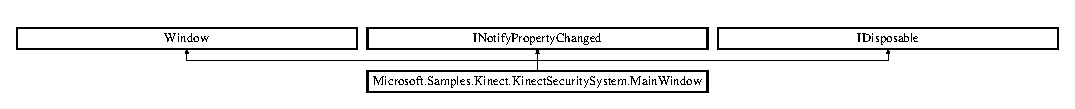
\includegraphics[height=1.022831cm]{class_microsoft_1_1_samples_1_1_kinect_1_1_kinect_security_system_1_1_main_window}
\end{center}
\end{figure}
\subsection*{Public Member Functions}
\begin{DoxyCompactItemize}
\item 
\hyperlink{class_microsoft_1_1_samples_1_1_kinect_1_1_kinect_security_system_1_1_main_window_a4ed9f24967289a072cf580d3d4cb19ba}{Main\+Window} ()
\begin{DoxyCompactList}\small\item\em Initializes a new instance of the \hyperlink{class_microsoft_1_1_samples_1_1_kinect_1_1_kinect_security_system_1_1_main_window}{Main\+Window} class \end{DoxyCompactList}\item 
void \hyperlink{class_microsoft_1_1_samples_1_1_kinect_1_1_kinect_security_system_1_1_main_window_a1b863ab898e2358e99993c0c30678e63}{Dispose} ()
\begin{DoxyCompactList}\small\item\em Disposes all unmanaged resources for the class \end{DoxyCompactList}\end{DoxyCompactItemize}
\subsection*{Protected Member Functions}
\begin{DoxyCompactItemize}
\item 
virtual void \hyperlink{class_microsoft_1_1_samples_1_1_kinect_1_1_kinect_security_system_1_1_main_window_a39200cb7da268b1502bca94a7d9146a0}{Dispose} (bool disposing)
\begin{DoxyCompactList}\small\item\em Disposes the \hyperlink{class_microsoft_1_1_samples_1_1_kinect_1_1_kinect_security_system_1_1_gesture_detector}{Gesture\+Detector} object \end{DoxyCompactList}\end{DoxyCompactItemize}
\subsection*{Properties}
\begin{DoxyCompactItemize}
\item 
string \hyperlink{class_microsoft_1_1_samples_1_1_kinect_1_1_kinect_security_system_1_1_main_window_a46bd6cf62b1d6706fb5fa49d24c42b1b}{Status\+Text}\hspace{0.3cm}{\ttfamily  \mbox{[}get\mbox{]}}
\begin{DoxyCompactList}\small\item\em Gets the current \hyperlink{namespace_microsoft_1_1_samples_1_1_kinect}{Kinect} sensor status text to display in UI \end{DoxyCompactList}\end{DoxyCompactItemize}
\subsection*{Events}
\begin{DoxyCompactItemize}
\item 
Property\+Changed\+Event\+Handler \hyperlink{class_microsoft_1_1_samples_1_1_kinect_1_1_kinect_security_system_1_1_main_window_afcc73bf291a2e49345083cf63d79078e}{Property\+Changed}
\begin{DoxyCompactList}\small\item\em I\+Notify\+Property\+Changed\+Property\+Changed event to allow window controls to bind to changeable data \end{DoxyCompactList}\end{DoxyCompactItemize}


\subsection{Detailed Description}
Interaction logic for the \hyperlink{class_microsoft_1_1_samples_1_1_kinect_1_1_kinect_security_system_1_1_main_window}{Main\+Window} 



\subsection{Constructor \& Destructor Documentation}
\mbox{\Hypertarget{class_microsoft_1_1_samples_1_1_kinect_1_1_kinect_security_system_1_1_main_window_a4ed9f24967289a072cf580d3d4cb19ba}\label{class_microsoft_1_1_samples_1_1_kinect_1_1_kinect_security_system_1_1_main_window_a4ed9f24967289a072cf580d3d4cb19ba}} 
\index{Microsoft\+::\+Samples\+::\+Kinect\+::\+Kinect\+Security\+System\+::\+Main\+Window@{Microsoft\+::\+Samples\+::\+Kinect\+::\+Kinect\+Security\+System\+::\+Main\+Window}!Main\+Window@{Main\+Window}}
\index{Main\+Window@{Main\+Window}!Microsoft\+::\+Samples\+::\+Kinect\+::\+Kinect\+Security\+System\+::\+Main\+Window@{Microsoft\+::\+Samples\+::\+Kinect\+::\+Kinect\+Security\+System\+::\+Main\+Window}}
\subsubsection{\texorpdfstring{Main\+Window()}{MainWindow()}}
{\footnotesize\ttfamily Microsoft.\+Samples.\+Kinect.\+Kinect\+Security\+System.\+Main\+Window.\+Main\+Window (\begin{DoxyParamCaption}{ }\end{DoxyParamCaption})}



Initializes a new instance of the \hyperlink{class_microsoft_1_1_samples_1_1_kinect_1_1_kinect_security_system_1_1_main_window}{Main\+Window} class 



\subsection{Member Function Documentation}
\mbox{\Hypertarget{class_microsoft_1_1_samples_1_1_kinect_1_1_kinect_security_system_1_1_main_window_a1b863ab898e2358e99993c0c30678e63}\label{class_microsoft_1_1_samples_1_1_kinect_1_1_kinect_security_system_1_1_main_window_a1b863ab898e2358e99993c0c30678e63}} 
\index{Microsoft\+::\+Samples\+::\+Kinect\+::\+Kinect\+Security\+System\+::\+Main\+Window@{Microsoft\+::\+Samples\+::\+Kinect\+::\+Kinect\+Security\+System\+::\+Main\+Window}!Dispose@{Dispose}}
\index{Dispose@{Dispose}!Microsoft\+::\+Samples\+::\+Kinect\+::\+Kinect\+Security\+System\+::\+Main\+Window@{Microsoft\+::\+Samples\+::\+Kinect\+::\+Kinect\+Security\+System\+::\+Main\+Window}}
\subsubsection{\texorpdfstring{Dispose()}{Dispose()}\hspace{0.1cm}{\footnotesize\ttfamily [1/2]}}
{\footnotesize\ttfamily void Microsoft.\+Samples.\+Kinect.\+Kinect\+Security\+System.\+Main\+Window.\+Dispose (\begin{DoxyParamCaption}{ }\end{DoxyParamCaption})}



Disposes all unmanaged resources for the class 

\mbox{\Hypertarget{class_microsoft_1_1_samples_1_1_kinect_1_1_kinect_security_system_1_1_main_window_a39200cb7da268b1502bca94a7d9146a0}\label{class_microsoft_1_1_samples_1_1_kinect_1_1_kinect_security_system_1_1_main_window_a39200cb7da268b1502bca94a7d9146a0}} 
\index{Microsoft\+::\+Samples\+::\+Kinect\+::\+Kinect\+Security\+System\+::\+Main\+Window@{Microsoft\+::\+Samples\+::\+Kinect\+::\+Kinect\+Security\+System\+::\+Main\+Window}!Dispose@{Dispose}}
\index{Dispose@{Dispose}!Microsoft\+::\+Samples\+::\+Kinect\+::\+Kinect\+Security\+System\+::\+Main\+Window@{Microsoft\+::\+Samples\+::\+Kinect\+::\+Kinect\+Security\+System\+::\+Main\+Window}}
\subsubsection{\texorpdfstring{Dispose()}{Dispose()}\hspace{0.1cm}{\footnotesize\ttfamily [2/2]}}
{\footnotesize\ttfamily virtual void Microsoft.\+Samples.\+Kinect.\+Kinect\+Security\+System.\+Main\+Window.\+Dispose (\begin{DoxyParamCaption}\item[{bool}]{disposing }\end{DoxyParamCaption})\hspace{0.3cm}{\ttfamily [protected]}, {\ttfamily [virtual]}}



Disposes the \hyperlink{class_microsoft_1_1_samples_1_1_kinect_1_1_kinect_security_system_1_1_gesture_detector}{Gesture\+Detector} object 


\begin{DoxyParams}{Parameters}
{\em disposing} & True if Dispose was called directly, false if the GC handles the disposing\\
\hline
\end{DoxyParams}


\subsection{Property Documentation}
\mbox{\Hypertarget{class_microsoft_1_1_samples_1_1_kinect_1_1_kinect_security_system_1_1_main_window_a46bd6cf62b1d6706fb5fa49d24c42b1b}\label{class_microsoft_1_1_samples_1_1_kinect_1_1_kinect_security_system_1_1_main_window_a46bd6cf62b1d6706fb5fa49d24c42b1b}} 
\index{Microsoft\+::\+Samples\+::\+Kinect\+::\+Kinect\+Security\+System\+::\+Main\+Window@{Microsoft\+::\+Samples\+::\+Kinect\+::\+Kinect\+Security\+System\+::\+Main\+Window}!Status\+Text@{Status\+Text}}
\index{Status\+Text@{Status\+Text}!Microsoft\+::\+Samples\+::\+Kinect\+::\+Kinect\+Security\+System\+::\+Main\+Window@{Microsoft\+::\+Samples\+::\+Kinect\+::\+Kinect\+Security\+System\+::\+Main\+Window}}
\subsubsection{\texorpdfstring{Status\+Text}{StatusText}}
{\footnotesize\ttfamily string Microsoft.\+Samples.\+Kinect.\+Kinect\+Security\+System.\+Main\+Window.\+Status\+Text\hspace{0.3cm}{\ttfamily [get]}}



Gets the current \hyperlink{namespace_microsoft_1_1_samples_1_1_kinect}{Kinect} sensor status text to display in UI 



\subsection{Event Documentation}
\mbox{\Hypertarget{class_microsoft_1_1_samples_1_1_kinect_1_1_kinect_security_system_1_1_main_window_afcc73bf291a2e49345083cf63d79078e}\label{class_microsoft_1_1_samples_1_1_kinect_1_1_kinect_security_system_1_1_main_window_afcc73bf291a2e49345083cf63d79078e}} 
\index{Microsoft\+::\+Samples\+::\+Kinect\+::\+Kinect\+Security\+System\+::\+Main\+Window@{Microsoft\+::\+Samples\+::\+Kinect\+::\+Kinect\+Security\+System\+::\+Main\+Window}!Property\+Changed@{Property\+Changed}}
\index{Property\+Changed@{Property\+Changed}!Microsoft\+::\+Samples\+::\+Kinect\+::\+Kinect\+Security\+System\+::\+Main\+Window@{Microsoft\+::\+Samples\+::\+Kinect\+::\+Kinect\+Security\+System\+::\+Main\+Window}}
\subsubsection{\texorpdfstring{Property\+Changed}{PropertyChanged}}
{\footnotesize\ttfamily Property\+Changed\+Event\+Handler Microsoft.\+Samples.\+Kinect.\+Kinect\+Security\+System.\+Main\+Window.\+Property\+Changed}



I\+Notify\+Property\+Changed\+Property\+Changed event to allow window controls to bind to changeable data 



The documentation for this class was generated from the following file\+:\begin{DoxyCompactItemize}
\item 
Kinect\+Security\+System/Main\+Window.\+xaml.\+cs\end{DoxyCompactItemize}

\hypertarget{class_microsoft_1_1_samples_1_1_kinect_1_1_kinect_security_system_1_1_robot_control}{}\section{Microsoft.\+Samples.\+Kinect.\+Kinect\+Security\+System.\+Robot\+Control Class Reference}
\label{class_microsoft_1_1_samples_1_1_kinect_1_1_kinect_security_system_1_1_robot_control}\index{Microsoft.\+Samples.\+Kinect.\+Kinect\+Security\+System.\+Robot\+Control@{Microsoft.\+Samples.\+Kinect.\+Kinect\+Security\+System.\+Robot\+Control}}


Holds the logic for controlling the robot arm using skeleton tracking  


Inheritance diagram for Microsoft.\+Samples.\+Kinect.\+Kinect\+Security\+System.\+Robot\+Control\+:\begin{figure}[H]
\begin{center}
\leavevmode
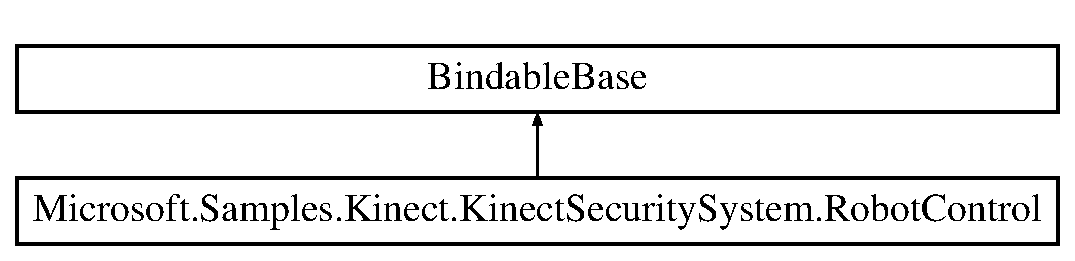
\includegraphics[height=2.000000cm]{class_microsoft_1_1_samples_1_1_kinect_1_1_kinect_security_system_1_1_robot_control}
\end{center}
\end{figure}
\subsection*{Public Member Functions}
\begin{DoxyCompactItemize}
\item 
\hyperlink{class_microsoft_1_1_samples_1_1_kinect_1_1_kinect_security_system_1_1_robot_control_acd1a271344cf99d83ddf38f50b49fdb9}{Robot\+Control} (\hyperlink{class_microsoft_1_1_samples_1_1_kinect_1_1_kinect_security_system_1_1_gesture_result_view}{Gesture\+Result\+View} view, string kinect\+Axis)
\begin{DoxyCompactList}\small\item\em Opens the serial and connects to the Arduino \end{DoxyCompactList}\item 
void \hyperlink{class_microsoft_1_1_samples_1_1_kinect_1_1_kinect_security_system_1_1_robot_control_aa66c741083e13b1720ffbd5e848ddd4b}{update\+Arm\+Data} (Body body)
\begin{DoxyCompactList}\small\item\em Update the position of the arm so we can move the servo arm \end{DoxyCompactList}\end{DoxyCompactItemize}
\subsection*{Properties}
\begin{DoxyCompactItemize}
\item 
string \hyperlink{class_microsoft_1_1_samples_1_1_kinect_1_1_kinect_security_system_1_1_robot_control_a14489e9305524cc1a7e22e2d5fd022e5}{Kinect\+Axis}\hspace{0.3cm}{\ttfamily  \mbox{[}get, set\mbox{]}}
\begin{DoxyCompactList}\small\item\em Gets or sets the value indicating which axis of the robot arm to control \end{DoxyCompactList}\end{DoxyCompactItemize}


\subsection{Detailed Description}
Holds the logic for controlling the robot arm using skeleton tracking 

\subsection{Constructor \& Destructor Documentation}
\mbox{\Hypertarget{class_microsoft_1_1_samples_1_1_kinect_1_1_kinect_security_system_1_1_robot_control_acd1a271344cf99d83ddf38f50b49fdb9}\label{class_microsoft_1_1_samples_1_1_kinect_1_1_kinect_security_system_1_1_robot_control_acd1a271344cf99d83ddf38f50b49fdb9}} 
\index{Microsoft\+::\+Samples\+::\+Kinect\+::\+Kinect\+Security\+System\+::\+Robot\+Control@{Microsoft\+::\+Samples\+::\+Kinect\+::\+Kinect\+Security\+System\+::\+Robot\+Control}!Robot\+Control@{Robot\+Control}}
\index{Robot\+Control@{Robot\+Control}!Microsoft\+::\+Samples\+::\+Kinect\+::\+Kinect\+Security\+System\+::\+Robot\+Control@{Microsoft\+::\+Samples\+::\+Kinect\+::\+Kinect\+Security\+System\+::\+Robot\+Control}}
\subsubsection{\texorpdfstring{Robot\+Control()}{RobotControl()}}
{\footnotesize\ttfamily Microsoft.\+Samples.\+Kinect.\+Kinect\+Security\+System.\+Robot\+Control.\+Robot\+Control (\begin{DoxyParamCaption}\item[{\hyperlink{class_microsoft_1_1_samples_1_1_kinect_1_1_kinect_security_system_1_1_gesture_result_view}{Gesture\+Result\+View}}]{view,  }\item[{string}]{kinect\+Axis }\end{DoxyParamCaption})}



Opens the serial and connects to the Arduino 



\subsection{Member Function Documentation}
\mbox{\Hypertarget{class_microsoft_1_1_samples_1_1_kinect_1_1_kinect_security_system_1_1_robot_control_aa66c741083e13b1720ffbd5e848ddd4b}\label{class_microsoft_1_1_samples_1_1_kinect_1_1_kinect_security_system_1_1_robot_control_aa66c741083e13b1720ffbd5e848ddd4b}} 
\index{Microsoft\+::\+Samples\+::\+Kinect\+::\+Kinect\+Security\+System\+::\+Robot\+Control@{Microsoft\+::\+Samples\+::\+Kinect\+::\+Kinect\+Security\+System\+::\+Robot\+Control}!update\+Arm\+Data@{update\+Arm\+Data}}
\index{update\+Arm\+Data@{update\+Arm\+Data}!Microsoft\+::\+Samples\+::\+Kinect\+::\+Kinect\+Security\+System\+::\+Robot\+Control@{Microsoft\+::\+Samples\+::\+Kinect\+::\+Kinect\+Security\+System\+::\+Robot\+Control}}
\subsubsection{\texorpdfstring{update\+Arm\+Data()}{updateArmData()}}
{\footnotesize\ttfamily void Microsoft.\+Samples.\+Kinect.\+Kinect\+Security\+System.\+Robot\+Control.\+update\+Arm\+Data (\begin{DoxyParamCaption}\item[{Body}]{body }\end{DoxyParamCaption})}



Update the position of the arm so we can move the servo arm 



\subsection{Property Documentation}
\mbox{\Hypertarget{class_microsoft_1_1_samples_1_1_kinect_1_1_kinect_security_system_1_1_robot_control_a14489e9305524cc1a7e22e2d5fd022e5}\label{class_microsoft_1_1_samples_1_1_kinect_1_1_kinect_security_system_1_1_robot_control_a14489e9305524cc1a7e22e2d5fd022e5}} 
\index{Microsoft\+::\+Samples\+::\+Kinect\+::\+Kinect\+Security\+System\+::\+Robot\+Control@{Microsoft\+::\+Samples\+::\+Kinect\+::\+Kinect\+Security\+System\+::\+Robot\+Control}!Kinect\+Axis@{Kinect\+Axis}}
\index{Kinect\+Axis@{Kinect\+Axis}!Microsoft\+::\+Samples\+::\+Kinect\+::\+Kinect\+Security\+System\+::\+Robot\+Control@{Microsoft\+::\+Samples\+::\+Kinect\+::\+Kinect\+Security\+System\+::\+Robot\+Control}}
\subsubsection{\texorpdfstring{Kinect\+Axis}{KinectAxis}}
{\footnotesize\ttfamily string Microsoft.\+Samples.\+Kinect.\+Kinect\+Security\+System.\+Robot\+Control.\+Kinect\+Axis\hspace{0.3cm}{\ttfamily [get]}, {\ttfamily [set]}}



Gets or sets the value indicating which axis of the robot arm to control 



The documentation for this class was generated from the following file\+:\begin{DoxyCompactItemize}
\item 
Kinect\+Security\+System/Robot\+Control.\+cs\end{DoxyCompactItemize}

%--- End generated contents ---

% Index
\backmatter
\newpage
\phantomsection
\clearemptydoublepage
\addcontentsline{toc}{chapter}{Index}
\printindex

\end{document}
